% openany: start chapters on the next page instead of the next right-hand
% page, so there are no blank pages between sections.
\documentclass[openany]{tietreport}

% Import images
\usepackage{graphicx}

% Fonts (T1 so braces and underscores in \texttt render correctly)
\usepackage[T1]{fontenc}
\usepackage{lmodern}

% Tables, figures and lists used in this report
\usepackage{booktabs}
\usepackage{longtable}
\usepackage{array}
\usepackage{float}
\usepackage{caption}
\usepackage{subcaption}
\usepackage{enumitem}
\setlist{nosep}
\usepackage[table]{xcolor}
\usepackage{pgfplots}
\pgfplotsset{compat=1.18}
\hypersetup{hidelinks}

\captionsetup{font=small}
\renewcommand{\arraystretch}{1.15}
\setlength{\emergencystretch}{3em}
\newcolumntype{L}[1]{>{\raggedright\arraybackslash}p{#1}}
\newcommand{\code}[1]{\texttt{\small #1}}
\newcommand{\pass}{\textbf{Pass}}
\newcommand{\fail}{\textbf{\textcolor{red!70!black}{Fail}}}

% Bibliography configuration
\usepackage[
  date=year,
  style=alphabetic,
  backend=biber,
  sorting=nty,
  maxnames=5,
  minnames=3,
  maxalphanames=4,
  minalphanames=3,
  backref=true,
  doi=false,
  isbn=false,
  url=false,
  eprint=false
]{biblatex}
\addbibresource{references.bib}

%% ==================================================
%% CUSTOMIZE THESE FIELDS FOR YOUR PROJECT
%% ==================================================

% Course/Lab header
\TitlePageHeader{%
  UCS503P Software Engineering Project Report%
}

% Main project title
\ProjectTitle{%
  CreditSetu%
}

% Subtitle or project description
\ProjectSubTitle{%
  A Dual-Path Credit Scoring and Lending Marketplace for Microfinance%
}

% Student information (up to 4 students)
\author{%
  \texttt{1024030564} Maanya Garg \\
  \texttt{1024030563} Kashvi Bansal \\
  \texttt{1024030565} Shreesh Gupta \\
  \texttt{1024031140} Shivam Raj%
}

% Group number, degree, year, program
\TitlePageSubText{%
  Group: \texttt{XXXX} BE Third Year, CSE%
}

% Faculty advisor/guide name
\AdvisorName{%
  Dr. Raghav B. Venkataramaiyer%
}

% Evaluation period and department info
\TitlePageFooterText{{%
    \large End-Semester Evaluation \\[0.2cm]
    \bfseries Computer Science and Engineering
    Department%
  } \\[0.15cm]
  Thapar Institute of Engineering and Technology,
  Patiala%
}

%% ==================================================

\begin{document}

% Generate title page
\maketitle

% ===== ABSTRACT =====
\chapter*{Abstract}
\addcontentsline{toc}{chapter}{Abstract}

CreditSetu is a credit-scoring and lending-marketplace platform for
microfinance in India. Every borrower builds an individual credit score
from their own repayment history. A borrower who belongs to a Self-Help
Group (SHG) starts from a head start earned by the group's track record,
while an independent borrower starts from a flat base of 450 and builds
purely from their own behaviour. Scores range from 300 to 900. They are
produced by an XGBoost classifier, explained feature by feature with SHAP,
and turned into plain-language improvement tips. Lenders partner with
specific SHGs through an explicit approve/reject linkage, and a
two-directional marketplace lets borrowers request loans (broadcast or
targeted) and lenders propose offers. Four separate role-gated logins
(Borrower, Lender, SHG, Admin) are authorised on the server, and a live
repayment flow with a demonstration wallet and payment gateway lets a
borrower's own payments move their own score.

This final report covers the requirements, the design, the implementation
and the evaluation of the complete system, including the work done after
the prototype stage. The most important late change is to the scoring
model: an investigation showed that the original, unconstrained model
could \emph{lower} a borrower's score after an on-time payment (in 18.8\%
of simulated cases). Retraining with monotone constraints, and removing a
feature that measured only the length of a borrower's history, reduced
this to 0\% at no cost in accuracy (5-fold cross-validated ROC-AUC 0.916,
against 0.915 before). On a single 95-borrower holdout the retrained model
reaches a ROC-AUC of 0.900 and an accuracy of 0.853. Running the
repayment flow end to end also exposed three defects, all fixed: fully
repaid loans that were still payable, missed instalments that could never
be cleared, and loans with no lender attached. All
measured read endpoints respond in a median of 5--28\,ms, and 169\,ms for
the heaviest lender query. The automated suite run at the prototype stage
passed 52 of 54 cases; its two low-severity defects remain open.

\vspace{1em}
\noindent\textbf{Keywords:} Microfinance, Credit Scoring, Cold Start,
XGBoost, Monotone Constraints, SHAP, Explainable AI, Self-Help Groups,
Role-Based Access Control, FastAPI, React.

% Table of contents (auto-generated from chapters)
\tableofcontents
\listoffigures
\listoftables

% ===== CHAPTER 1: INTRODUCTION =====

\chapter{Introduction}

\section{Background and Context}

Microfinance is one of the main routes to formal credit for low-income
households in India, and much of it runs through Self-Help Groups: small
groups, often of women, who save together, meet regularly and borrow with
shared responsibility. Lending decisions in this setting still depend
largely on group reputation and on the judgement of field staff. A credit
bureau score is of little help, because most of these borrowers have never
held a formal loan.

CreditSetu is a software system that gives each of these borrowers an
individual, explainable credit score and connects them with lenders
through a controlled marketplace. Figure~\ref{fig:overview} gives an
overview of the approach.

\begin{figure}[H]
\centering
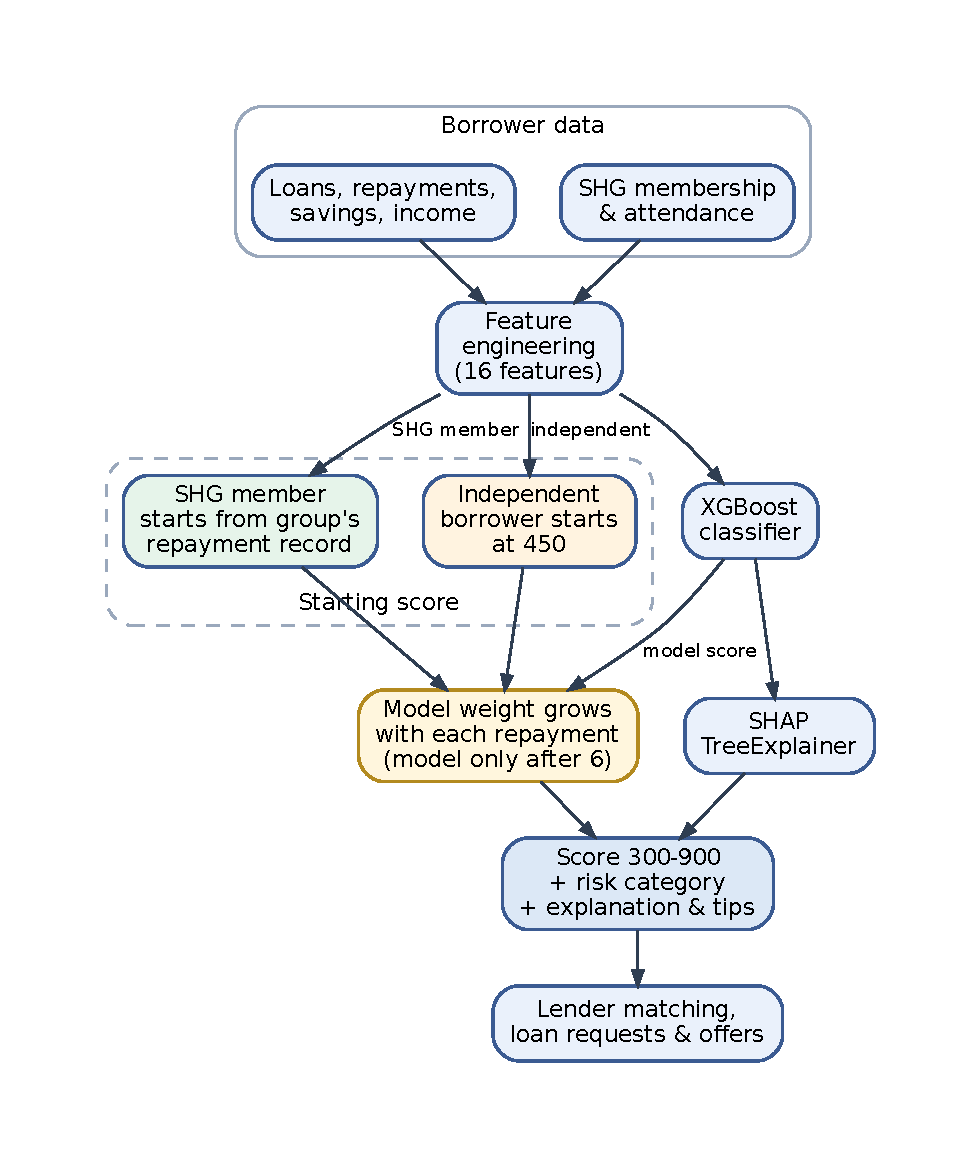
\includegraphics[width=0.62\textwidth]{fig/overview.pdf}
\caption{Overview of the dual-path scoring approach used in CreditSetu}
\label{fig:overview}
\end{figure}

An earlier version of this project (\texttt{Sahara MFI}, a Node/Express
and MySQL application) scored only SHG members, through a hand-written SQL
formula, with no path for independent borrowers, no machine learning and
no lender marketplace. CreditSetu is a from-scratch rebuild: the domain
(SHGs, loans, repayments, credit scores) carries over, but the schema, the
scoring approach and the system design are new.

\subsection{Problem Statement}

\begin{itemize}
  \item \textbf{Cold-start scoring:} a borrower with no formal credit
  history cannot be scored by a model that learns only from past
  repayments. This hits independent borrowers hardest, because they have
  no group record to fall back on.
  \item \textbf{Opaque scoring:} where a score exists it is usually a
  single number with no reason attached. A borrower cannot tell what to
  improve, and a lender cannot check whether the score makes sense.
  \item \textbf{No formal SHG--lender relationship:} lending at group
  level is informal, unauditable and cannot be revoked cleanly.
  \item \textbf{Undifferentiated access:} in an open system a borrower, a
  lender and an SHG all see the same data.
\end{itemize}

\section{Project Objectives}

Table~\ref{tab:objectives} lists the objectives set at the proposal stage
and how far each one has been met. Section~\ref{sec:analysis} discusses
them in detail.

\begin{table}[H]
\centering
\caption{Project objectives and their status at the final evaluation}
\label{tab:objectives}
\small
\begin{tabular}{@{}lL{6.6cm}L{5.0cm}@{}}
\toprule
\textbf{\#} & \textbf{Objective} & \textbf{Status and evidence}\\
\midrule
O1 & Dual-path scoring: SHG members get a group-earned head start, independent borrowers build a score from their own behaviour & Met. Exactly 450 for a new independent borrower; group-based start for SHG members (Section~\ref{sec:scoring})\\
O2 & Every score explained feature by feature with SHAP and turned into improvement tips & Met. Stored per score, in score points\\
O3 & Formal SHG--lender approve/reject linkage & Met. Only the non-initiating party can decide\\
O4 & Four role-gated views, authorised on the server & Met, with one open status-code defect (D-02)\\
O5 & A borrower's own repayments move their own score through a live flow & Met. Verified end to end on 18~Nov~2026 (Section~\ref{sec:finalrun})\\
O6 & Scoring model with holdout ROC-AUC $\ge 0.85$ and accuracy $\ge 0.80$ & Met. 0.900 and 0.853\\
O7 & Read endpoints answer in a median below 300\,ms & Met. 5--169\,ms (Table~\ref{tab:perf})\\
O8 & Validate the system with an automated test suite & Met at the prototype stage (52/54). The suite is not in the repository and was not rerun\\
\bottomrule
\end{tabular}
\end{table}

\section{Motivation}

Groups that repay reliably have already shown the discipline a lender
cares about. CreditSetu lets that record give each member a fair starting
point, and then lets each member's own repayments take over. Borrowers
without a group should still be able to build a score from nothing, and
both kinds of borrower should be told what is affecting their score. The
project also meets the course selection criteria: it can be delivered in
weekly increments, it is locally relevant, and it can be built entirely
with mature open-source tools.

\section{Related Work}
\label{sec:related}

Traditional microfinance credit assessment relies heavily on group
liability and on manual judgement by field agents, with little use of
statistical or machine-learning scoring. Formal credit bureaus such as
CIBIL score individuals who already have a formal credit history, and
offer no way for a first-time, group-affiliated borrower to inherit a
trust signal from their group. Commercial microfinance information
systems, including the team's own earlier \texttt{Sahara MFI} build,
typically implement a single SHG-only scoring formula with no cold-start
path and no explanation of the result.

Gradient-boosted decision trees, and XGBoost~\cite{xgboost} in
particular, are a standard choice for tabular credit-risk data: they
handle missing values natively, need little feature scaling and train in
seconds on datasets of this size. XGBoost can also be told that a feature
may only push the prediction in one direction (a \emph{monotone
constraint}~\cite{monotone}), which matters in credit scoring, where a
worse repayment record must never produce a better score. Explainable-AI
techniques such as SHAP~\cite{shap,treeshap} are increasingly used in
consumer credit scoring in developed markets, but much less in
microfinance tooling. Isolation Forest~\cite{iforest} and
$k$-means~\cite{kmeans} are established methods for outlier detection and
for grouping regions by behaviour.

What is missing in the existing work is the combination. CreditSetu treats
the cold-start problem and model opacity together: an explicit blend from
a starting score to the model, weighted by how much of the borrower's own
history exists, and an explanation that covers the starting score as well
as the model.

\section{Organisation of the Report}

Chapter~\ref{ch:method} gives the requirements and the design and
describes each implemented module. Chapter~\ref{ch:results} reports the
dataset, the model's performance, the investigation and fix of the score's
response to a single payment, the end-to-end validation of the repayment
flow, response times and testing. Chapter~\ref{ch:concl} concludes and
lists the remaining work. The use case diagram with its scenarios, the
class diagram and the activity diagrams are in
Appendices~\ref{app:usecase}--\ref{app:activity}.

% ===== CHAPTER 2: METHODOLOGY & DESIGN =====

\chapter{Methodology and Design}
\label{ch:method}

\section{Requirements}

\subsection{Stakeholders}

Table~\ref{tab:actors} lists the four user roles. Each role has its own
login and its own dashboard.

\begin{table}[H]
\centering
\caption{User roles and their responsibilities}
\label{tab:actors}
\small
\begin{tabular}{@{}L{2.6cm}L{10.6cm}@{}}
\toprule
\textbf{Role} & \textbf{Responsibilities in CreditSetu}\\
\midrule
Borrower & View own score, history, explanation and tips; request loans; accept or reject offers; repay EMIs.\\
Self-Help Group & View group statistics and member scores; request or approve partnerships with lenders.\\
Lender & View reputation score; browse SHGs; manage partnerships; see eligible borrowers; make offers; approve or decline loan requests.\\
Admin (Bank) & Read-only oversight: portfolio summary, district clusters, anomaly flags, model health and borrower search.\\
\bottomrule
\end{tabular}
\end{table}

\subsection{Functional Requirements}

The requirements below follow the structure of IEEE Std~830~\cite{ieee830}.
FR2 and FR8 were revised after the prototype stage; the changes are noted
in the table.

\begin{table}[H]
\centering
\caption{Functional requirements}
\label{tab:fr}
\small
\begin{tabular}{@{}lL{12.2cm}@{}}
\toprule
\textbf{ID} & \textbf{Requirement}\\
\midrule
FR1 & Provide separate logins for Borrower, Lender, SHG and Admin, and enforce role and ownership checks on the server (401 or 403).\\
FR2 & Compute a 300--900 score for every borrower from 15 engineered model features, using the dual-path starting score when there is little or no history. \emph{(Revised: 16 features at the prototype stage.)}\\
FR3 & Store every score as a new history row with its SHAP explanation, and show up to five improvement tips.\\
FR4 & Let a borrower create, retarget and withdraw loan requests; a targeted request is visible only to its target lender.\\
FR5 & Let a lender approve (with an interest rate) or decline a request; approval creates an active loan, and a decline does not close the request for other lenders.\\
FR6 & Let a lender propose offers to eligible borrowers within its maximum loan amount; the borrower accepts or rejects.\\
FR7 & Manage SHG--lender partnerships; only the party that did not start the request may decide it.\\
FR8 & Calculate each loan's EMI, let the borrower pay any loan whose EMI the wallet covers, and record the repayment and the rescore in one transaction. \emph{(Revised: the prototype blocked every payment unless the wallet covered the total due across all loans.)}\\
FR9 & Give the admin a portfolio summary, district clusters, anomaly detection, model health and borrower search.\\
\bottomrule
\end{tabular}
\end{table}

\subsection{Non-Functional Requirements}

\begin{table}[H]
\centering
\caption{Non-functional requirements and target values}
\label{tab:nfr}
\small
\begin{tabular}{@{}lL{2.6cm}L{9.6cm}@{}}
\toprule
\textbf{ID} & \textbf{Category} & \textbf{Requirement}\\
\midrule
NFR1 & Performance & Median response time of read endpoints below 300\,ms on the demonstration dataset.\\
NFR2 & Security & 100\% of cross-role or cross-identity requests refused; passwords stored only as salted hashes.\\
NFR3 & Accuracy & Scoring model holdout ROC-AUC at least 0.85 and accuracy at least 0.80.\\
NFR4 & Reliability & A payment and its rescore are atomic: a failed request leaves no partial change.\\
NFR5 & Scalability & Switch from SQLite to PostgreSQL through \code{DATABASE\_URL} only; all foreign keys indexed; list endpoints paginated.\\
NFR6 & Usability & Plain-language explanations; text-size, high-contrast and dark-mode controls.\\
NFR7 & Privacy & Only synthetic data; the public home page shows aggregate highlights only.\\
NFR8 & Consistency & A worse repayment record must never produce a better score, all else equal. \emph{(Added after the prototype stage; see Section~\ref{sec:monotone}.)}\\
\bottomrule
\end{tabular}
\end{table}

\section{System Architecture}

\subsection{High-Level Design}

CreditSetu is a three-tier web application with an offline machine-learning
pipeline:

\begin{itemize}
  \item \textbf{Frontend:} a React single-page application with a public
  landing page and four role-gated dashboards. It is styled as a
  government-portal-style \emph{demonstration} platform and clearly
  labelled as such.
  \item \textbf{Backend API:} FastAPI~\cite{fastapi}, exposing REST
  endpoints under \code{/api} through twelve routers. Every request is
  authenticated with a per-role bearer token, and every query is scoped on
  the server to the caller's own identity. Routers delegate to service
  modules, which are the only place business rules live.
  \item \textbf{Database:} SQLAlchemy over SQLite for the demonstration. A
  single \code{DATABASE\_URL} setting moves it to PostgreSQL with no code
  changes.
  \item \textbf{ML pipeline:} command-line scripts for synthetic data
  generation, model training and batch scoring, plus one-off idempotent
  migration scripts. They produce artifacts that the API loads once at
  start-up; nothing is trained at request time.
\end{itemize}

\subsection{Technical Stack}

\begin{table}[H]
\centering
\caption{Technology stack}
\label{tab:stack}
\small
\begin{tabular}{@{}L{3.2cm}L{10cm}@{}}
\toprule
\textbf{Layer} & \textbf{Technology}\\
\midrule
Frontend & React 19 single-page application, Vite, React Router, Recharts\\
Backend & Python 3.11, FastAPI 0.115 (REST API with OpenAPI docs), Uvicorn\\
Database & SQLAlchemy 2.0 ORM over SQLite (demonstration); PostgreSQL through a configuration setting\\
Machine learning & XGBoost 2.1, SHAP 0.46, scikit-learn 1.5~\cite{sklearn} ($k$-means, Isolation Forest), pandas, NumPy\\
Data & Synthetic borrower population generated with Faker (seed 42)\\
Testing & pytest, FastAPI TestClient, Playwright (prototype-stage suite); scripted end-to-end checks with curl and a real browser (final stage)\\
Tools & Git and GitHub, GitHub Actions (documentation site), PlantUML and Graphviz (diagrams), \LaTeX{}\\
\bottomrule
\end{tabular}
\end{table}

\subsection{Data Model}

The schema has 19 tables. Its core is \code{districts}, \code{shgs} and
\code{individuals}, where \code{individuals.shg\_id} is the dual-path
pivot: it is nullable, and NULL means the borrower is independent. Around
this sit the attendance and savings records, \code{lenders},
\code{shg\_lender\_links} (the approve/reject partnership table, which
records which side initiated each link), \code{loans},
\code{repayment\_events}, \code{credit\_scores} (append-only score
history), \code{score\_explanations} (one row per feature contribution per
score), \code{loan\_offers} and \code{loan\_requests} (the two directions
of the marketplace), \code{anomaly\_flags} and one session table per role.
Each borrower also has a \code{wallet\_balance} for the demonstration
payment flow. Every foreign key is indexed. The class diagram in
Appendix~\ref{app:class} shows every table and relationship.

\section{Implementation Details}

\subsection{Module 1: Scoring Engine}
\label{sec:scoring}

Each borrower's score is computed in five steps, shown as an activity
diagram in Appendix~\ref{app:activity}, Figure~\ref{fig:activity}.

\begin{enumerate}
  \item \textbf{Build features.} The borrower's loans, repayments,
  savings, income and (for SHG members) meeting attendance are turned into
  15 model features, such as the on-time, late, partial and missed
  repayment rates, the average days late and savings regularity. Missing
  data is marked as unknown rather than treated as zero, and is imputed at
  training and serving time with the same stored medians, so training and
  serving cannot drift apart.
  \item \textbf{Choose a starting score.} An SHG member starts from a
  score based on how well the \emph{other} members of the group repay
  (60\% weight on the group's record and 40\% on a neutral 500). An
  independent borrower starts from a flat 450.
  \item \textbf{Blend in the model.} With no repayments the starting score
  is used as it is, and the model is not called. With each repayment event
  more weight moves to the model's prediction, and after six events the
  model is used alone.
  \item \textbf{Explain.} SHAP contributions are converted into score
  points and stored as explanation rows, measured against the score of an
  average borrower rather than the floor of 300. This keeps the
  explanation meaningful for a borrower with a low score.
  \item \textbf{Assign a risk band and save.} The score is clipped to
  300--900 and labelled Very Low risk (800 or more), Low (700--799), Medium
  (550--699), High (450--549) or Very High (below 450). Every run appends a
  new score row; older scores are never overwritten.
\end{enumerate}

The model is an XGBoost classifier (200 trees, maximum depth 4, learning
rate 0.05, subsample and column-sample ratios 0.9) that predicts whether a
borrower has a defaulted loan. It is trained on SHG-linked borrowers with
at least three repayment events, using an 80/20 stratified split. Two
design decisions were added after the prototype stage, both explained in
Section~\ref{sec:monotone}:

\begin{itemize}
  \item \textbf{Monotone constraints.} More on-time repayment, savings
  regularity, attendance or peer repayment can only lower the predicted
  default risk; more late, partial or missed repayments, or more days late,
  can only raise it.
  \item \textbf{No history-length feature.} \code{n\_repayment\_events}
  is still computed, because it sets the blending weight in step~3, but it
  is no longer a model input.
\end{itemize}

\subsection{Module 2: Authentication and Access Control}

The four roles log in separately: phone and password for borrowers, and
username and password for the other three. Passwords are stored only as
salted PBKDF2-HMAC-SHA256 hashes~\cite{pbkdf2}. A successful login returns
a random opaque session token that expires after seven days. There is no
JWT and no client-side claim that the server trusts.

Every protected endpoint uses one of five FastAPI dependencies (one per
role, plus ``any logged-in role''). The borrower, lender or SHG a request
refers to is always taken from the session, never from the request body,
and any identifier in a URL is checked against what the session may see.
The server answers 401 when there is no valid token and 403 when the
caller is known but not entitled. Table~\ref{tab:rbac} summarises what each
role may see.

\begin{table}[H]
\centering
\caption{Data access matrix (enforced on the server)}
\label{tab:rbac}
\small
\begin{tabular}{@{}L{3.3cm}L{2.0cm}L{3.0cm}L{2.3cm}L{2.0cm}@{}}
\toprule
\textbf{Data} & \textbf{Borrower} & \textbf{Lender} & \textbf{SHG} & \textbf{Admin}\\
\midrule
Own score, history, SHAP & Own only & -- & -- & All (read)\\
Other borrowers & Denied & Linked SHGs or independents & Own members & All (read)\\
SHG details and members & Own SHG, no member list & Members if link Approved & Own SHG & All (read)\\
Loan requests and offers & Own & Addressed to or made by them & Denied & All (read)\\
Partnership decisions & Denied & SHG-initiated links & Lender-initiated links & Denied\\
Anomalies, clusters, model health & Denied & Denied & Denied & Allowed\\
\bottomrule
\end{tabular}
\end{table}

\subsection{Module 3: Loan Marketplace and Lender Reputation}

A lender is \emph{eligible} for a borrower if (i) the borrower's SHG has
an Approved link with the lender, or the borrower is independent and the
lender serves independent borrowers, and (ii) the borrower's latest score
is at least the lender's minimum. A borrower may broadcast a loan request
to every eligible lender or target one, and may retarget or withdraw a
pending request. A lender approves a request with an interest rate, which
creates an active loan, or declines it; a decline only removes the request
from that lender's queue. In the other direction a lender may propose an
offer to an eligible borrower within its maximum loan amount.

To reward competitive pricing, in the spirit of the Reserve Bank of
India's priority-sector and co-lending incentives~\cite{rbi}, each lender
has a reputation score from 0 to 100 (50 is the platform average). It
rises when the lender's base rate and the rates it actually offers are
below the platform average, and further with marketplace activity and
willingness to serve independent borrowers.

\subsection{Module 4: Repayment and Demonstration Payment Gateway}
\label{sec:repay}

Every borrower has a wallet, seeded at 1.5 times their monthly income. A
demonstration payment gateway, clearly labelled as not real and protected
by a fixed demonstration login, shows the wallet and the EMI due on each
active loan. The EMI is the principal plus simple interest over the full
tenure, divided equally across the months. Four rules decide what is due:

\begin{itemize}
  \item \textbf{Cycle number.} The next instalment is (number of
  repayment events already recorded on the loan) $+\,1$. Counting events
  rather than calendar time means a loan is payable as soon as it is
  disbursed. \emph{Every} recorded event counts, including Missed and
  Partial ones: a missed cycle is history, not a debt that blocks the loan
  for ever.
  \item \textbf{Nothing owed, nothing due.} A loan whose cycle has run
  past its tenure, or whose outstanding balance is already zero, is not
  offered for payment.
  \item \textbf{Per-loan sufficiency.} A payment is allowed when the
  wallet covers \emph{that loan's} EMI. The prototype blocked every
  payment unless the wallet covered the total across all loans; the team
  changed this so a borrower can pay the loans they can afford, in any
  order.
  \item \textbf{On time or late.} A payment made on or before the cycle's
  due date (disbursement date plus 30 days per cycle) is On\_Time;
  otherwise it is Late, with the number of days late recorded.
\end{itemize}

A payment reloads the wallet on the server, re-checks the rules above,
records the repayment event, debits the wallet, reduces the outstanding
balance, closes the loan after its last cycle or when the balance reaches
zero, and recomputes the credit score, all in one database transaction.
Each loan row on the repayment page names the lender being repaid.

\subsection{Module 5: Analytics for the Admin}

The admin dashboard groups the ten districts into trust levels with
$k$-means~\cite{kmeans} on their score and repayment statistics, labelling
each cluster by the rank of its mean score, and flags unusual borrowers
with an Isolation Forest~\cite{iforest}. Clusters are recomputed on each
request, which is cheap for ten districts. The admin also sees a portfolio
summary, model health and borrower search.

% ===== CHAPTER 3: RESULTS & EVALUATION =====

\chapter{Results and Evaluation}
\label{ch:results}

Unless a date is given, every figure in this chapter was measured on the
running system on 18~November~2026, on a Windows~11 machine with 16
logical processors and 15.3\,GB of memory, using Python~3.11.9.

\section{Dataset}

Because real borrower data is sensitive, the system uses a reproducible
synthetic population (Table~\ref{tab:data}). Defaults follow a smooth
probabilistic rule based on missed, late and partial payments, not a hard
threshold. The seeded loan history originally had no lender attached and
some fully repaid loans were still marked active; both were corrected
(Section~\ref{sec:defects}).

\begin{table}[H]
\centering
\caption{Demonstration dataset at the time of writing}
\label{tab:data}
\small
\begin{tabular}{@{}lr@{\hskip 1.2cm}lr@{}}
\toprule
\textbf{Entity} & \textbf{Count} & \textbf{Entity} & \textbf{Count}\\
\midrule
Borrowers & 1{,}079 & Loans & 1{,}652\\
\quad SHG-linked & 659 & \quad Active & 672\\
\quad Independent & 420 & \quad Closed & 613\\
SHGs & 51 & \quad Defaulted & 367 (22.2\%)\\
Lenders & 6 & Repayment events & 16{,}993\\
Districts & 10 & \quad On time / Late & 10{,}986 / 2{,}353\\
SHG--lender links & 101 & \quad Partial / Missed & 1{,}583 / 2{,}071\\
Model training rows & 475 & Stored score rows (history) & 3{,}246\\
\bottomrule
\end{tabular}
\end{table}

\section{Scoring Model Performance}

Table~\ref{tab:model} gives the performance of the final model and its most
important features, measured as mean absolute SHAP value. Missed-payment
rate dominates, as expected; the number of loans and the consistency and
regularity of savings come next.

\begin{table}[H]
\centering
\caption{Final scoring model: performance and top features}
\label{tab:model}
\small
\begin{tabular}{@{}lr@{\hskip 0.6cm}lr@{}}
\toprule
\textbf{Metric} & \textbf{Value} & \textbf{Feature} & \textbf{Mean $|$SHAP$|$}\\
\midrule
Holdout ROC-AUC & 0.900 & \code{missed\_rate} & 1.61\\
Holdout accuracy & 0.853 & \code{n\_loans} & 0.59\\
5-fold CV ROC-AUC & 0.916 & \code{savings\_consistency} & 0.58\\
Precision / recall (default) & 0.75 / 0.75 & \code{avg\_days\_late} & 0.48\\
Training rows (default rate) & 475 (29.9\%) & \code{savings\_regularity} & 0.43\\
Holdout size & 95 (28 defaults) & \code{on\_time\_rate} & 0.39\\
\bottomrule
\end{tabular}
\end{table}

Both NFR3 targets are met. The holdout figures are lower than the
prototype report's (ROC-AUC 0.962, accuracy 0.909), which were measured on
an earlier data snapshot with the unconstrained model. A single holdout of
95 borrowers, of whom only 28 defaulted, is a noisy measure. For that
reason the comparison between model variants in
Section~\ref{sec:monotone} uses 5-fold cross-validation on the same data.

Figure~\ref{fig:dist} shows the latest score of every borrower by risk
band. SHG-linked borrowers average 688.4 and independent borrowers 650.2.
Of the 420 independent borrowers, 97 have no repayment history yet and sit
at exactly 450, in the High-risk band. That is the dual-path design working
as intended: they start lower and build from their own record. In total
310 borrowers (29\%) still carry some weight from their starting score.

\begin{figure}[H]
\centering
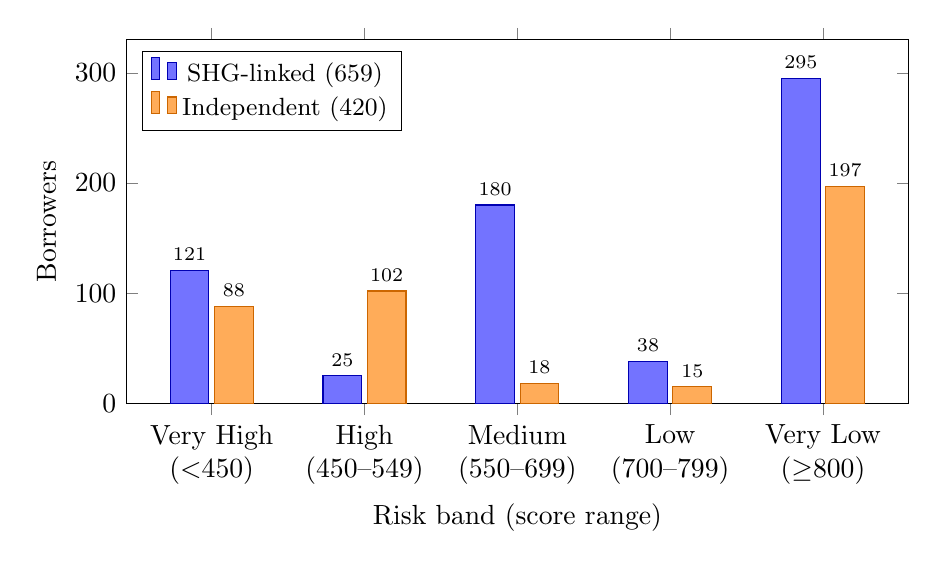
\begin{tikzpicture}
\begin{axis}[
  ybar, bar width=14pt, width=0.95\textwidth, height=6.2cm,
  ymin=0, ymax=330,
  symbolic x coords={Very High,High,Medium,Low,Very Low},
  xtick=data,
  xticklabel style={align=center},
  xticklabels={{Very High\\($<$450)},{High\\(450--549)},{Medium\\(550--699)},{Low\\(700--799)},{Very Low\\($\geq$800)}},
  ylabel={Borrowers},
  xlabel={Risk band (score range)},
  nodes near coords, nodes near coords style={font=\scriptsize},
  legend style={at={(0.02,0.97)}, anchor=north west, font=\small},
  enlarge x limits=0.14,
]
\addplot[fill=blue!55, draw=blue!70!black] coordinates
  {(Very High,121) (High,25) (Medium,180) (Low,38) (Very Low,295)};
\addplot[fill=orange!65, draw=orange!80!black] coordinates
  {(Very High,88) (High,102) (Medium,18) (Low,15) (Very Low,197)};
\legend{SHG-linked (659), Independent (420)}
\end{axis}
\end{tikzpicture}
\caption{Latest credit score of every borrower by risk band and path}
\label{fig:dist}
\end{figure}

\section{How the Score Responds to a Single Payment}
\label{sec:monotone}

\subsection{The Problem}

While testing the repayment flow, a borrower's score moved in ways that
did not match the payments: it fell from 852 to 848 after one late
payment, then rose to 860 after another, which was 179 days overdue. To
find out whether this was a bug or the model's behaviour, the score was
recomputed for the same borrowers with one extra On\_Time, Late or Missed
repayment added, without changing the database.

For one borrower, an On\_Time payment, a Late one at 5 days and a Late one
at 179 days all lowered the score by the same 5 points. Across 271
SHG-linked borrowers with at least six repayment events, the average
direction was right but individual results were not (first column of
Table~\ref{tab:mono}): an on-time payment lowered the score for 18.8\% of
borrowers.

\subsection{Causes}

\begin{enumerate}
  \item \textbf{No monotonicity.} The unconstrained model was free to
  learn any shape, and with only about 475 training rows it learned
  noise: for one borrower, raising \code{late\_rate} from 0.18 to 0.25
  \emph{raised} the score from 847 to 864.
  \item \textbf{A history-length feature.} \code{n\_repayment\_events}
  counts how many payments a borrower has made, not how well they paid.
  Every payment of any kind increases it by one, so a single extra event
  could move the score sharply. For the same borrower, going from 30 to 34
  events changed the score by 87 points.
\end{enumerate}

\subsection{The Fix and Its Effect}

Three model variants were compared with 5-fold cross-validation on the
same data: the original model (ROC-AUC 0.915), the same model with
monotone constraints (0.913), and the constrained model without
\code{n\_repayment\_events} (0.916). The last was adopted, the model was
retrained, and all 1{,}079 borrowers were rescored; their earlier score
history was kept. Table~\ref{tab:mono} compares the two models.

\begin{table}[H]
\centering
\caption{Effect of one extra repayment on 271 borrowers, before and after the fix}
\label{tab:mono}
\small
\begin{tabular}{@{}L{7.2cm}rr@{}}
\toprule
\textbf{Measure} & \textbf{Original model} & \textbf{Final model}\\
\midrule
Mean change after an On\_Time payment & $+4.9$ & $+6.5$\\
Mean change after a Late payment (30 days) & $-3.1$ & $-2.8$\\
Mean change after a Missed payment & $-31.1$ & $-30.2$\\
On\_Time payment \emph{lowers} the score & 18.8\% & \textbf{0\%}\\
Late payment scores \emph{higher} than On\_Time & 17.3\% & 5\%\\
Missed payment scores \emph{higher} than On\_Time & not measured & \textbf{0\%}\\
5-fold cross-validated ROC-AUC & 0.915 & 0.916\\
\bottomrule
\end{tabular}
\end{table}

Two limits remain. First, for about 68\% of borrowers a single extra
On\_Time payment changes nothing: one event is a small change to rates
built from dozens of events, and it often does not cross a split in a
model trained on 475 rows. Second, in 5\% of cases a Late payment still
scores slightly above an On\_Time one. These are mostly legitimate: a late
payment of fewer days than the borrower's own average lowers their
\code{avg\_days\_late}. NFR8 is therefore met for the two cases that matter
most: an on-time payment never lowers a score, and a missed payment never
scores better than an on-time one. The remaining late-payment cases are
explained by that dilution effect.

\section{End-to-End Validation of the Repayment Flow}
\label{sec:finalrun}

After all fixes were in place, the complete repayment flow was run on
18~November~2026 against a backup copy of the database, which was restored
afterwards. Table~\ref{tab:finalrun} lists the steps for one SHG-linked
borrower (wallet Rs.~14{,}272.50), first through the API and then through
the browser. Each step was checked against the database.

\begin{table}[H]
\centering
\caption{End-to-end repayment run, 18 November 2026}
\label{tab:finalrun}
\small
\begin{tabular}{@{}lL{4.6cm}L{4.4cm}l@{}}
\toprule
\textbf{Step} & \textbf{Action} & \textbf{Observed} & \textbf{Result}\\
\midrule
1 & API: open due summary & Two loans, each naming its lender; fully repaid loan not listed; next EMI \#18 of 24 & \pass\\
2 & API: pay the Rs.~1{,}074.41 EMI & Wallet 14{,}272.50 $\to$ 13{,}198.09; Late, 59 days; score 858 $\to$ 849 & \pass\\
3 & API: pay the closed loan & 400 ``This loan isn't active'' & \pass\\
4 & API: pay or view another borrower's loan & 403 & \pass\\
5 & API: unknown loan; no token & 404; 401 & \pass\\
6 & API: wallet Rs.~774.71 against Rs.~1{,}293.50 due & 400 \code{insufficient\_funds} with both amounts & \pass\\
7 & Browser: log in, open Repay, sign in to gateway & Shows wallet 13{,}198.09 and EMI \#19 from step~2 & \pass\\
8 & Browser: pay the Rs.~2{,}052.66 EMI & ``Paid -- Late''; wallet 11{,}145.43; EMI \#6 $\to$ \#7 & \pass\\
9 & Database check & Two new Late events (59 and 46 days), balances reduced, two rescore rows & \pass\\
\bottomrule
\end{tabular}
\end{table}

The server log showed no errors (HTTP 500). The only 401 and 403 responses
were the application's own check for an existing session before login and
the deliberate negative tests above. The run covered one borrower through
the browser and one more for the insufficient-funds case; it is a
validation of the flow, not of the whole population.

\section{Performance Metrics}

Table~\ref{tab:perf} gives median response times over 21 requests per
endpoint, measured over \code{127.0.0.1} to exclude a local name-resolution
delay of about 200\,ms that affects \code{localhost} on Windows. Login is
slow by design, because PBKDF2 runs 200{,}000 iterations.

\begin{table}[H]
\centering
\caption{Median API response times and targets}
\label{tab:perf}
\small
\begin{tabular}{@{}L{6.6cm}rrl@{}}
\toprule
\textbf{Endpoint} & \textbf{Median} & \textbf{Target} & \textbf{Result}\\
\midrule
\code{GET /api/payments/due-summary} & 5.3\,ms & $<300$\,ms & \pass\\
\code{GET /api/individuals/\{id\}} & 7.4\,ms & $<300$\,ms & \pass\\
\code{GET /api/dashboard/summary} & 8.6\,ms & $<300$\,ms & \pass\\
\code{GET /api/shgs} & 16.1\,ms & $<300$\,ms & \pass\\
\code{GET /api/geo/districts} ($k$-means each time) & 27.8\,ms & $<300$\,ms & \pass\\
\code{GET /api/lenders/\{id\}/\allowbreak eligible-borrowers} & 169.0\,ms & $<300$\,ms & \pass\\
\code{POST /api/auth/login} (PBKDF2) & 67.4\,ms & -- & --\\
\bottomrule
\end{tabular}
\end{table}

\section{Testing Methodology}

\begin{itemize}
  \item \textbf{Unit testing:} scoring formulas, risk-band boundaries and
  the reputation logic, with pytest (8 cases).
  \item \textbf{Integration testing:} REST endpoints called with real
  tokens for authentication, access control, the marketplace, payments,
  links, offers and analytics, with pytest and FastAPI's TestClient (38
  cases). These ran against a temporary copy of the database, and the
  borrower/lender pairs were chosen at run time from the current
  eligibility rules.
  \item \textbf{System testing:} user journeys in a real browser with
  Playwright (8 cases), and at the final stage the scripted end-to-end
  repayment run in Section~\ref{sec:finalrun}.
  \item \textbf{Performance testing:} median response times of the main
  endpoints (Table~\ref{tab:perf}).
  \item \textbf{Model behaviour testing:} the counterfactual
  single-payment analysis in Section~\ref{sec:monotone}.
\end{itemize}

Test cases were designed with equivalence partitioning (valid, invalid and
unauthorised inputs) and boundary value analysis (risk bands and the ends
of the score range), as described by Pressman and
Maxim~\cite{pressman}.

\section{Test Results}

The automated suite of 54 cases was run on 17~September~2026, at the
prototype stage. Its files are not in the project repository, so it could
not be rerun for this report; Table~\ref{tab:tc} reports that run as it
was. Three later changes affect it:

\begin{itemize}
  \item TC23 recorded ROC-AUC 0.962 and accuracy 0.909 for the earlier
  model. The final model's 0.900 and 0.853 still meet the same targets.
  \item TC32, TC34 and E2E06 were written for the aggregate wallet rule.
  Under the current per-loan rule, a payment is blocked only when the
  wallet cannot cover that loan's EMI (step~6 of
  Table~\ref{tab:finalrun}).
  \item The defects fixed after the prototype
  (Section~\ref{sec:defects}) were found by the end-to-end run, not by this
  suite, which did not cover them.
\end{itemize}

{\small
\begin{longtable}{@{}lL{1.6cm}L{4.0cm}L{2.5cm}L{2.4cm}l@{}}
\caption{Automated test cases and results (run of 17 September 2026)}\label{tab:tc}\\
\toprule
\textbf{ID} & \textbf{Module} & \textbf{Test case} & \textbf{Expected} & \textbf{Actual} & \textbf{Status}\\
\midrule
\endfirsthead
\toprule
\textbf{ID} & \textbf{Module} & \textbf{Test case} & \textbf{Expected} & \textbf{Actual} & \textbf{Status}\\
\midrule
\endhead
\bottomrule
\endfoot
TC01 & Auth & Borrower login with valid phone and password & 200 + token & 200, token issued & \pass\\
TC02 & Auth & Borrower login with wrong password & 401 & 401 & \pass\\
TC03 & Auth & Login with an unregistered phone number & 401 & 401 & \pass\\
TC04 & Auth & Lender, SHG and admin login (3 runs) & 200 each & 200 each & \pass\\
TC05 & Auth & Admin login with wrong password & 401 & 401 & \pass\\
TC06 & Auth & Protected endpoints called without a token & 401 & 401 & \pass\\
TC07 & Auth & Reuse a token after logout & 401 & 401 & \pass\\
TC08 & Auth & Each account has a uniquely salted hash & Different hashes & All 1{,}079 borrowers share one hash & \fail\\
TC09 & RBAC & Borrower reads another borrower's record & 403 & 403 & \pass\\
TC10 & RBAC & Borrower calls admin-only borrower list & 403 & 401 (still denied) & \fail\\
TC11 & RBAC & Admin lists the population & 200 & 200 & \pass\\
TC12 & RBAC & Lender opens an unlinked SHG & 403 & 403 & \pass\\
TC13 & RBAC & Lender opens an approved-linked SHG & 200 with members & 200 with members & \pass\\
TC14 & RBAC & Borrower opens own SHG & Summary, no members & As expected & \pass\\
TC15 & RBAC & Anomaly flags for borrower vs admin & Denied / 200 & Denied / 200 & \pass\\
TC16 & RBAC & Public home highlights without login & 200 & 200 & \pass\\
TC17 & Scoring & New independent borrower (0 repayments) & Exactly 450 & 450 & \pass\\
TC18 & Scoring & New SHG member (0 repayments) & Group-based start, above 450 & As expected & \pass\\
TC19 & Scoring & All stored scores within range & 300--900 & In range & \pass\\
TC20 & Scoring & Explanation rows add up to score $-$ 300 & Within tolerance & Within tolerance & \pass\\
TC21 & Scoring & Risk band at 9 boundary scores & Correct band & 9/9 correct & \pass\\
TC22 & Scoring & Probability-to-score conversion & 300, 600, 900 at ends and middle & As expected & \pass\\
TC23 & Scoring & Model quality targets & AUC $\ge$0.85, acc.\ $\ge$0.80 & 0.962 / 0.909 & \pass\\
TC24 & Requests & Principal = 0 & 400 & 400 & \pass\\
TC25 & Requests & Target an ineligible lender & 400 & 400 & \pass\\
TC26 & Requests & Targeted request visibility & Only target lender & Only target lender & \pass\\
TC27 & Requests & Lender declines a broadcast request & Still Pending & Pending, hidden from that lender & \pass\\
TC28 & Requests & Approve without an interest rate & 400 & 400 & \pass\\
TC29 & Requests & Approve with rate 12\% & Active loan created & Loan Active, balance 6{,}000 & \pass\\
TC30 & Requests & Withdraw the same request twice & Withdrawn, then 400 & As expected & \pass\\
TC31 & Requests & Withdraw another borrower's request & 403 & 403 & \pass\\
TC32 & Payments & Due-summary totals & Sum of EMIs & Consistent & \pass\\
TC33 & Payments & Pay EMI (Rs.~6{,}000, 12\%, 6 months) & Rs.~1{,}060 paid, On\_Time, new score & Exactly as expected & \pass\\
TC34 & Payments & Wallet of Rs.~1 & 400, nothing changed & 400, balance unchanged & \pass\\
TC35 & Payments & Pay another borrower's loan & 403 & 403 & \pass\\
TC36 & Links & SHG requests; SHG self-approves; lender approves & Pending; 403; Approved & As expected & \pass\\
TC37 & Links & Duplicate partnership request & 400 & 400 & \pass\\
TC38 & Links & Re-decide an approved link & 400 & 400 & \pass\\
TC39 & Links & Admin tries to decide a link & 403 & 403 & \pass\\
TC40 & Offers & Offer to an ineligible borrower & 400 & 400 & \pass\\
TC41 & Offers & Offer above the maximum loan amount & 400 & 400 & \pass\\
TC42 & Offers & Wrong borrower, then right borrower, accepts & 403; loan created & As expected & \pass\\
TC43 & Analytics & Lower base rate increases reputation & Higher score & Higher score & \pass\\
TC44 & Analytics & Best district is labelled High Trust & Correct label & Correct & \pass\\
TC45 & Analytics & Dashboard counts add up & Consistent & Consistent & \pass\\
TC46 & Perf. & Median time of \code{GET /api/shgs} & $<300$\,ms & $\approx$13\,ms & \pass\\
E2E01 & UI & Borrower login opens own dashboard & Welcome + SHAP card & Shown & \pass\\
E2E02 & UI & Wrong password message & ``Incorrect credentials.'' & Shown & \pass\\
E2E03 & UI & Open /admin without a session & Redirect to login & Redirected & \pass\\
E2E04 & UI & Borrower session opens /lender & Lender data not shown & Not shown & \pass\\
E2E05 & UI & Pay an EMI from the Repay page & ``New score'' shown & Shown & \pass\\
E2E06 & UI & Repay with a wallet of Rs.~5 & Blocked banner & Shown & \pass\\
E2E07 & UI & Lender dashboard content & Reputation + requests & Shown & \pass\\
E2E08 & UI & Log out, then open /shg & Redirect to login & Redirected & \pass\\
\end{longtable}
}

\begin{table}[H]
\centering
\caption{Test summary by module (run of 17 September 2026)}
\label{tab:summary}
\small
\begin{tabular}{@{}lccccL{3.5cm}@{}}
\toprule
\textbf{Module} & \textbf{Cases} & \textbf{Pass} & \textbf{Fail} & \textbf{Rate} & \textbf{Observation}\\
\midrule
Authentication & 11 & 10 & 1 & 90.9\% & Shared seeded hash (D-01)\\
Access control & 10 & 9 & 1 & 90.0\% & 401 instead of 403 (D-02)\\
Scoring engine & 7 & 7 & 0 & 100\% & Starting scores exact\\
Loan requests & 8 & 8 & 0 & 100\% & Rules enforced on the server\\
Payments & 6 & 6 & 0 & 100\% & Atomic\\
Partnerships and offers & 7 & 7 & 0 & 100\% & Only the correct party decides\\
Analytics and performance & 5 & 5 & 0 & 100\% & \\
\midrule
\textbf{Total} & \textbf{54} & \textbf{52} & \textbf{2} & \textbf{96.3\%} & \\
\bottomrule
\end{tabular}
\end{table}

\section{Defects}
\label{sec:defects}

\subsection{Fixed After the Prototype Stage}

The end-to-end run of the repayment flow and the investigation of the
score found four defects, all fixed (Table~\ref{tab:fixed}). Each fix was
checked against the database and applied to existing data with an
idempotent migration script; running each script a second time changed
nothing.

\begin{table}[H]
\centering
\caption{Defects found and fixed after the prototype stage}
\label{tab:fixed}
\small
\begin{tabular}{@{}L{6.4cm}L{6.8cm}@{}}
\toprule
\textbf{Defect} & \textbf{Cause and fix}\\
\midrule
64 loans had a zero balance but stayed Active, and the Repay page offered to charge a full EMI on them & The data generator tracked balances as principal only, so loans reached zero before their last cycle. Loans now close at a zero balance; existing data migrated\\
A Missed cycle stayed ``due'' for ever, with a due date that contradicted the Missed record & The cycle counter ignored Missed and Partial events. Every recorded event now resolves its cycle\\
An on-time payment lowered the score for 18.8\% of borrowers & Unconstrained model and a history-length feature. Monotone constraints; feature removed; model retrained (Section~\ref{sec:monotone})\\
The Repay page could not say which lender was being repaid (1{,}644 of 1{,}652 loans had none) & Seeded loans had no lender. They are now attributed to a lender the marketplace rules allow (0 rule violations); 38 loans whose SHG has no approved lender show ``Lender not recorded''\\
\bottomrule
\end{tabular}
\end{table}

Earlier defects, fixed before the prototype report, included inverted
$k$-means cluster labels, an empty SHAP explanation for high-risk
borrowers, a broken partnership approve button, and an N+1 query on the
SHG list that made it 75 times slower than necessary.

\subsection{Open Defects}

Both defects found by the automated suite are still present; this was
checked in the code on 18~November~2026.

\begin{table}[H]
\centering
\caption{Open defects}
\label{tab:open}
\small
\begin{tabular}{@{}lL{5.6cm}L{1.6cm}L{4.8cm}@{}}
\toprule
\textbf{ID} & \textbf{Description} & \textbf{Severity} & \textbf{Recommended fix}\\
\midrule
D-01 & The data generator hashes the demonstration password once, so all 1{,}079 seeded borrowers share one salt and hash. & Low (demo data) & Call \code{hash\_password()} once per borrower.\\
D-02 & Admin-only endpoints answer 401 to a valid token of another role instead of 403. Access is still denied. & Low & Return 403 in \code{get\_current\_admin} for another role's valid session.\\
\bottomrule
\end{tabular}
\end{table}

\section{User Interface}

Figures~\ref{fig:ui1} and~\ref{fig:ui2} show screens from the running
application, captured at the prototype stage. The Repay page now also
names the lender on each loan, and the ``payment blocked'' screen
reflects the earlier aggregate wallet rule.

\begin{figure}[H]
\centering
\begin{subfigure}[t]{0.49\textwidth}\centering
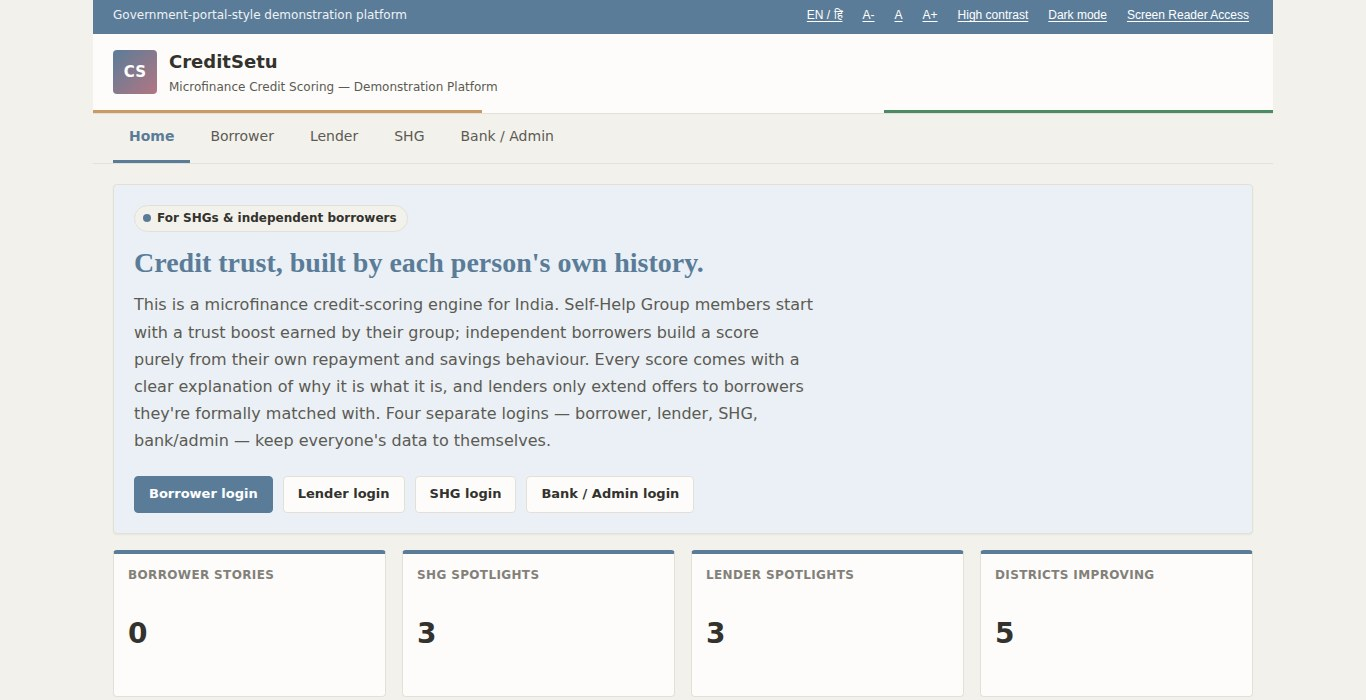
\includegraphics[width=\textwidth]{shots/ss_home_hero.jpg}
\caption{Public home page with role logins}
\end{subfigure}\hfill
\begin{subfigure}[t]{0.49\textwidth}\centering
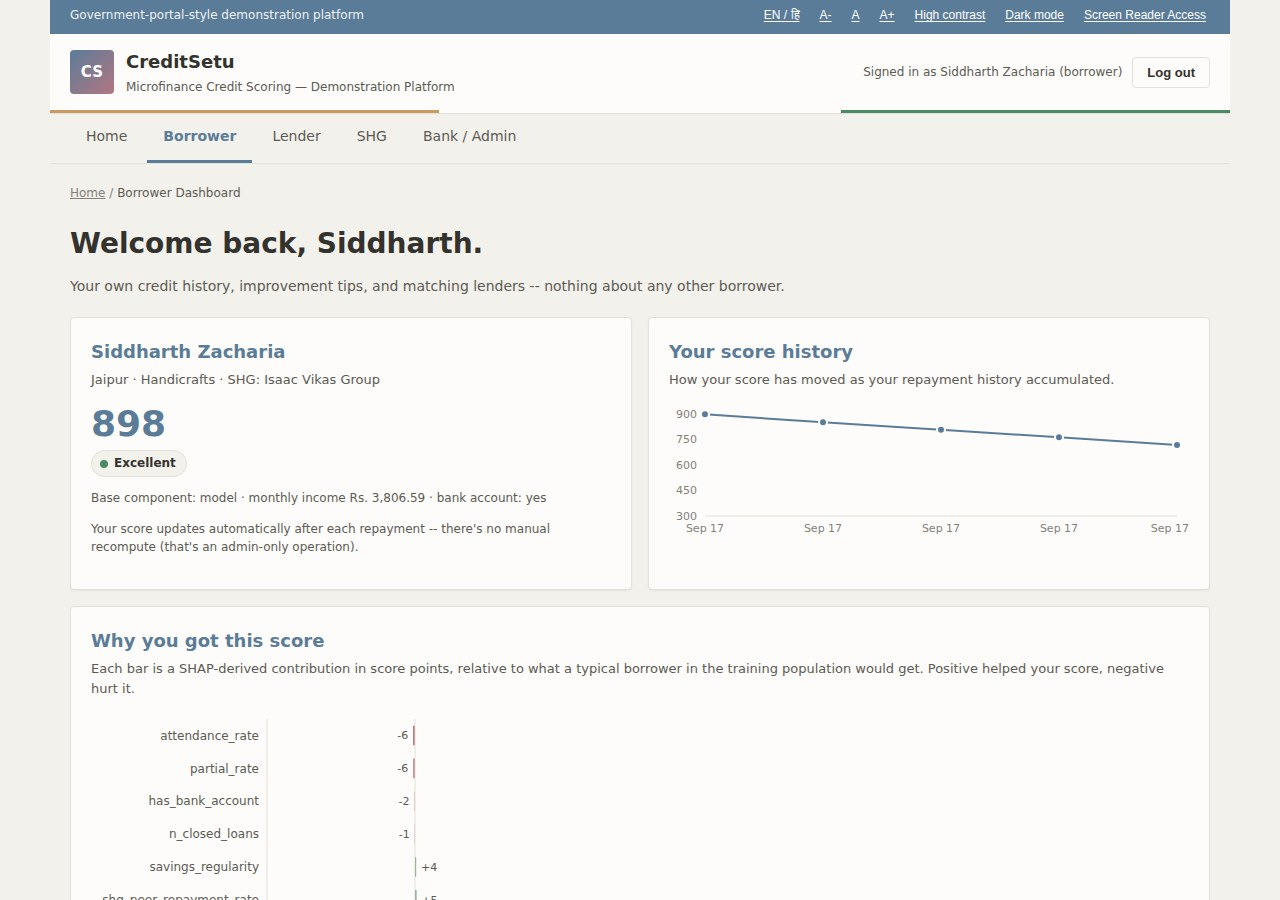
\includegraphics[width=\textwidth]{shots/ss_b_top.jpg}
\caption{Borrower dashboard and score history}
\end{subfigure}\\[6pt]
\begin{subfigure}[t]{0.49\textwidth}\centering
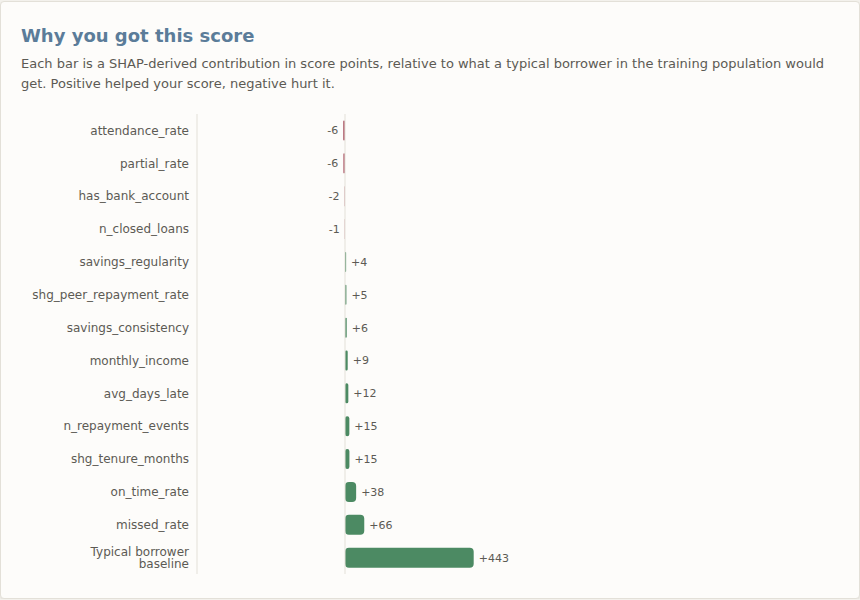
\includegraphics[width=\textwidth]{shots/b_shap.png}
\caption{``Why you got this score'' (SHAP)}
\end{subfigure}\hfill
\begin{subfigure}[t]{0.49\textwidth}\centering
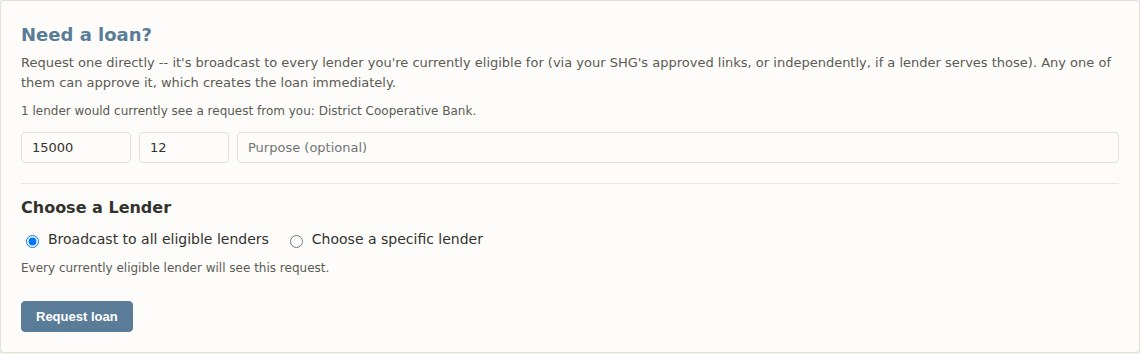
\includegraphics[width=\textwidth]{shots/ss_b_need.jpg}
\caption{Loan request (broadcast or targeted)}
\end{subfigure}\\[6pt]
\begin{subfigure}[t]{0.24\textwidth}\centering
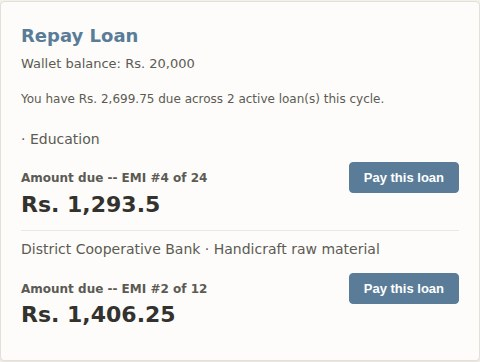
\includegraphics[width=\textwidth]{shots/ss_pay_before.jpg}
\caption{Repay page}
\end{subfigure}\hfill
\begin{subfigure}[t]{0.24\textwidth}\centering
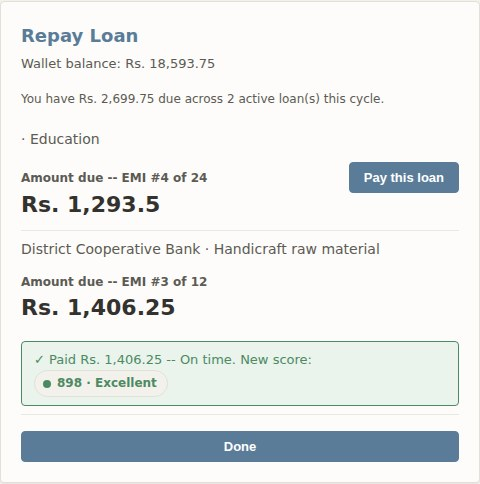
\includegraphics[width=\textwidth]{shots/ss_pay_after.jpg}
\caption{After payment}
\end{subfigure}\hfill
\begin{subfigure}[t]{0.49\textwidth}\centering
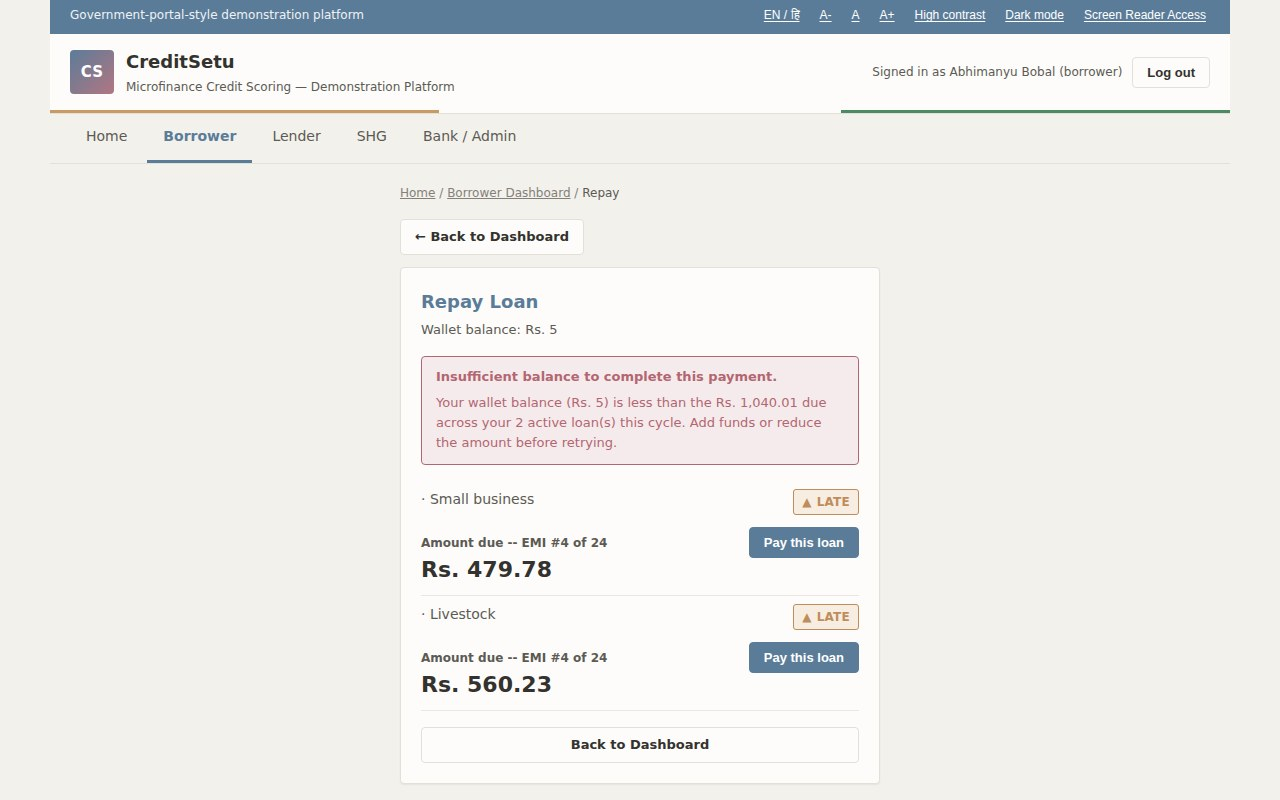
\includegraphics[width=\textwidth]{shots/ss_pay_blocked.jpg}
\caption{Payment blocked (earlier aggregate rule)}
\end{subfigure}
\caption{Borrower screens}
\label{fig:ui1}
\end{figure}

\begin{figure}[H]
\centering
\begin{subfigure}[t]{0.49\textwidth}\centering
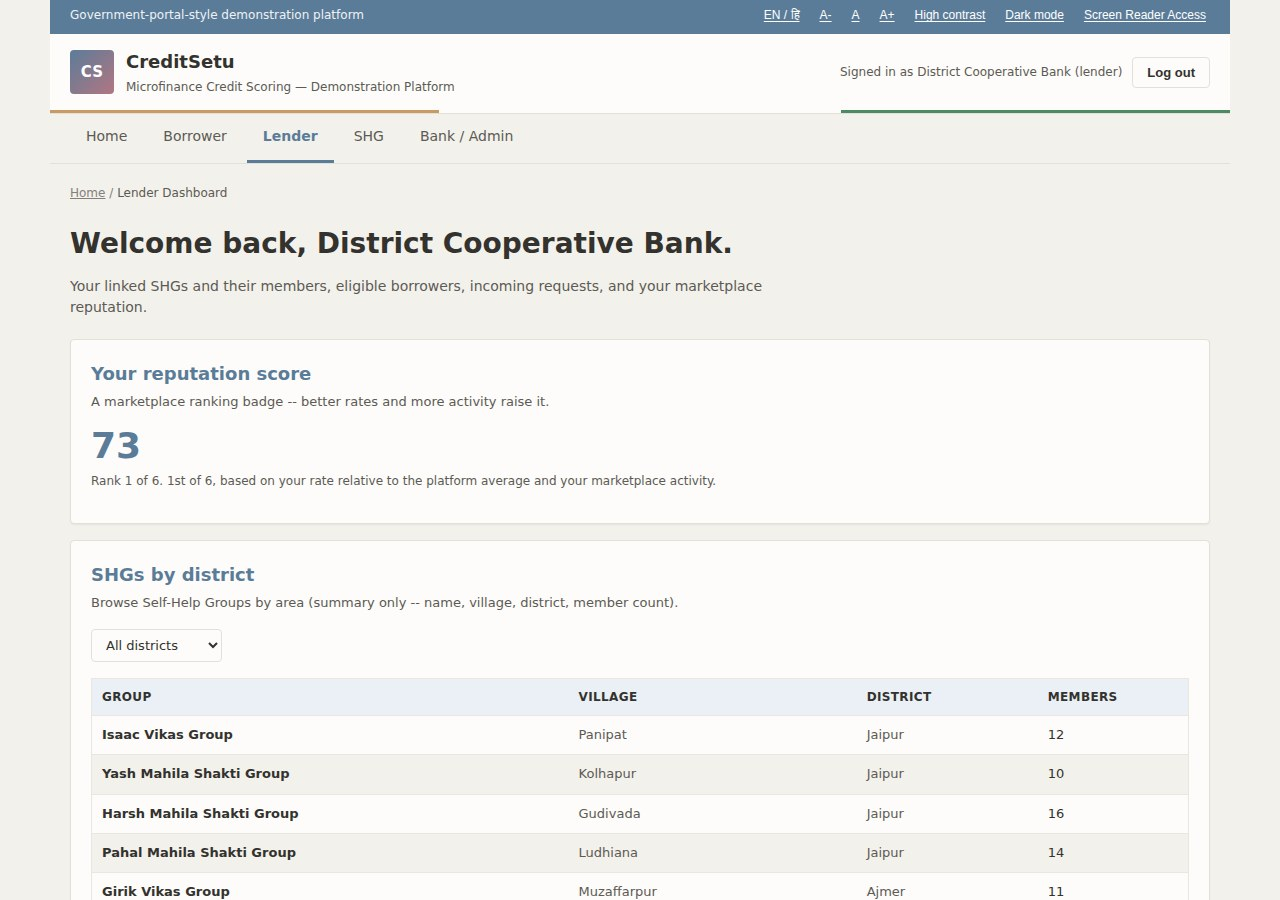
\includegraphics[width=\textwidth]{shots/ss_l_top.jpg}
\caption{Lender dashboard with reputation}
\end{subfigure}\hfill
\begin{subfigure}[t]{0.49\textwidth}\centering
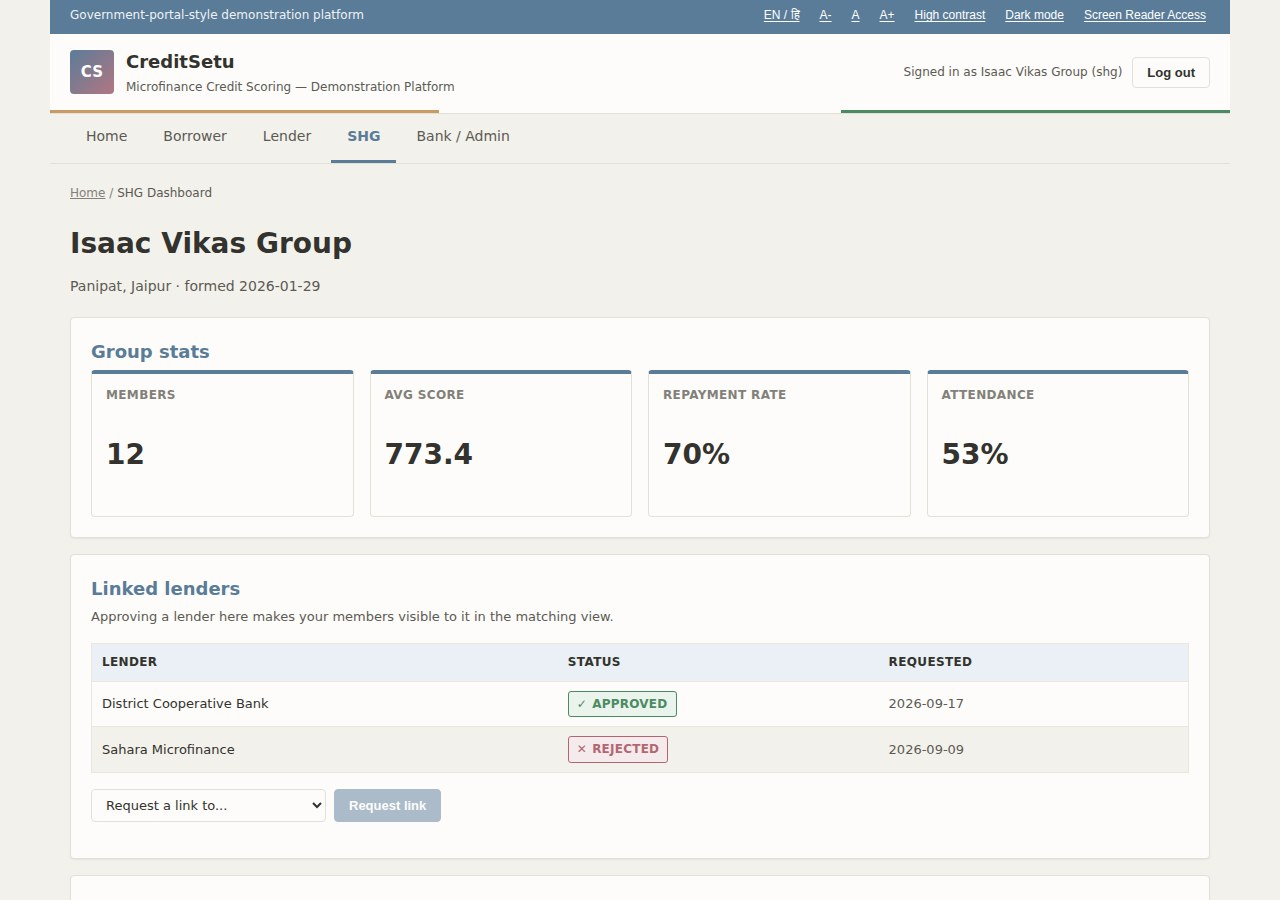
\includegraphics[width=\textwidth]{shots/ss_s_top.jpg}
\caption{SHG dashboard}
\end{subfigure}\\[6pt]
\begin{subfigure}[t]{0.49\textwidth}\centering
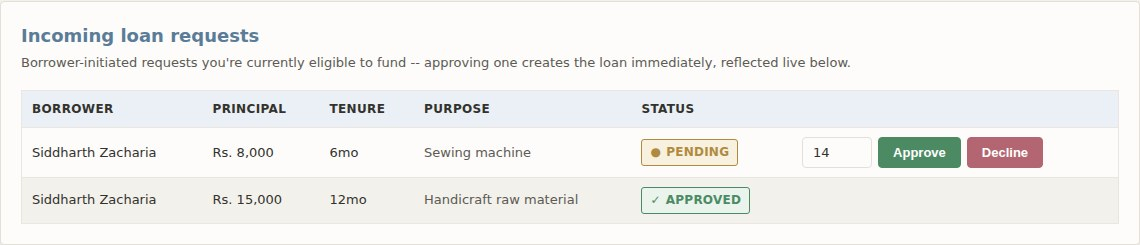
\includegraphics[width=\textwidth]{shots/ss_l_in.jpg}
\caption{Lender: incoming loan requests}
\end{subfigure}\hfill
\begin{subfigure}[t]{0.49\textwidth}\centering
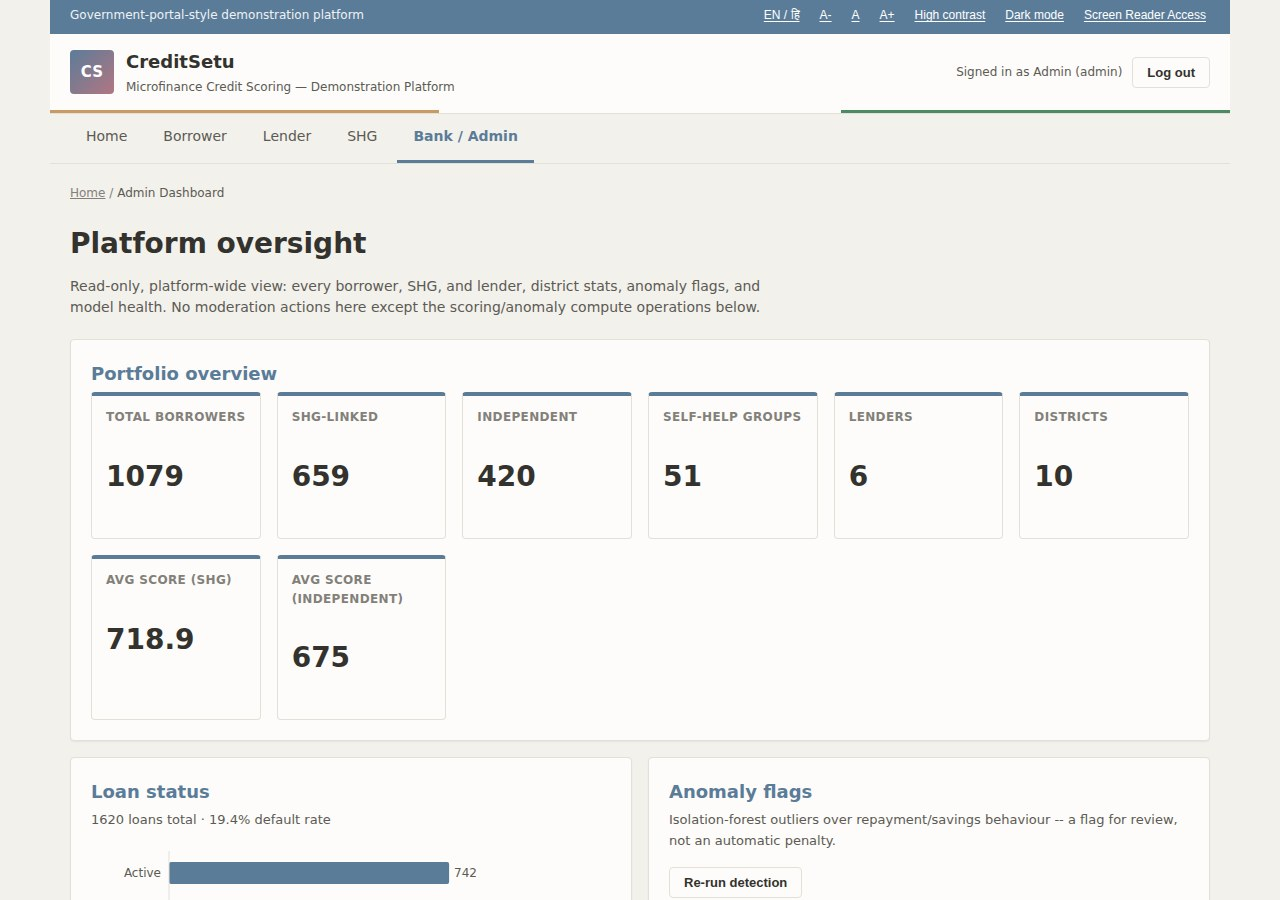
\includegraphics[width=\textwidth]{shots/ss_a_top.jpg}
\caption{Admin: platform overview}
\end{subfigure}\\[6pt]
\begin{subfigure}[t]{0.49\textwidth}\centering
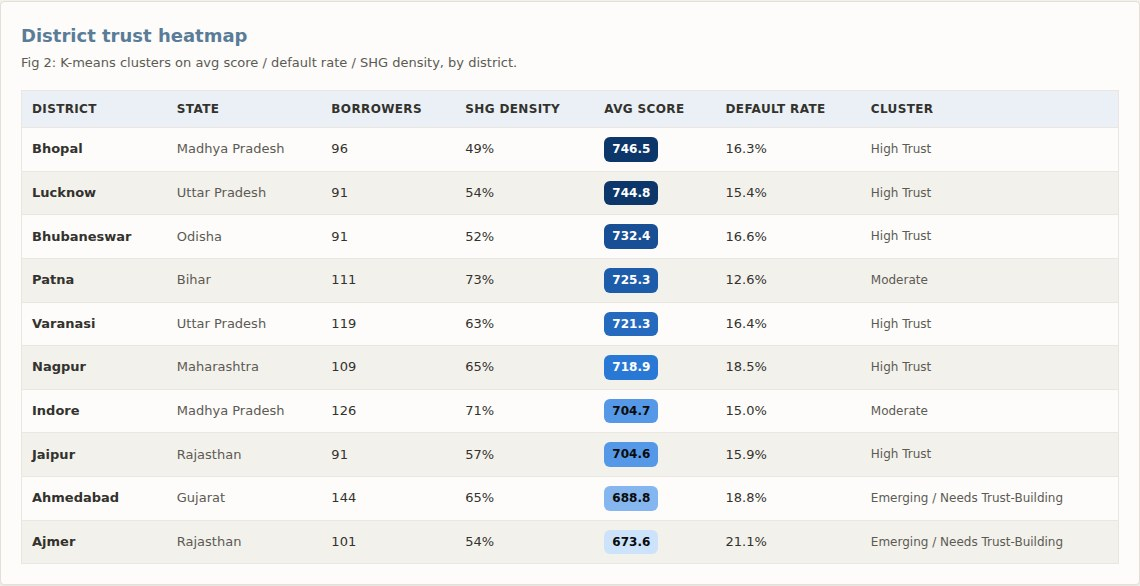
\includegraphics[width=\textwidth]{shots/ss_a_heat.jpg}
\caption{Admin: district trust heatmap}
\end{subfigure}\hfill
\begin{subfigure}[t]{0.49\textwidth}\centering
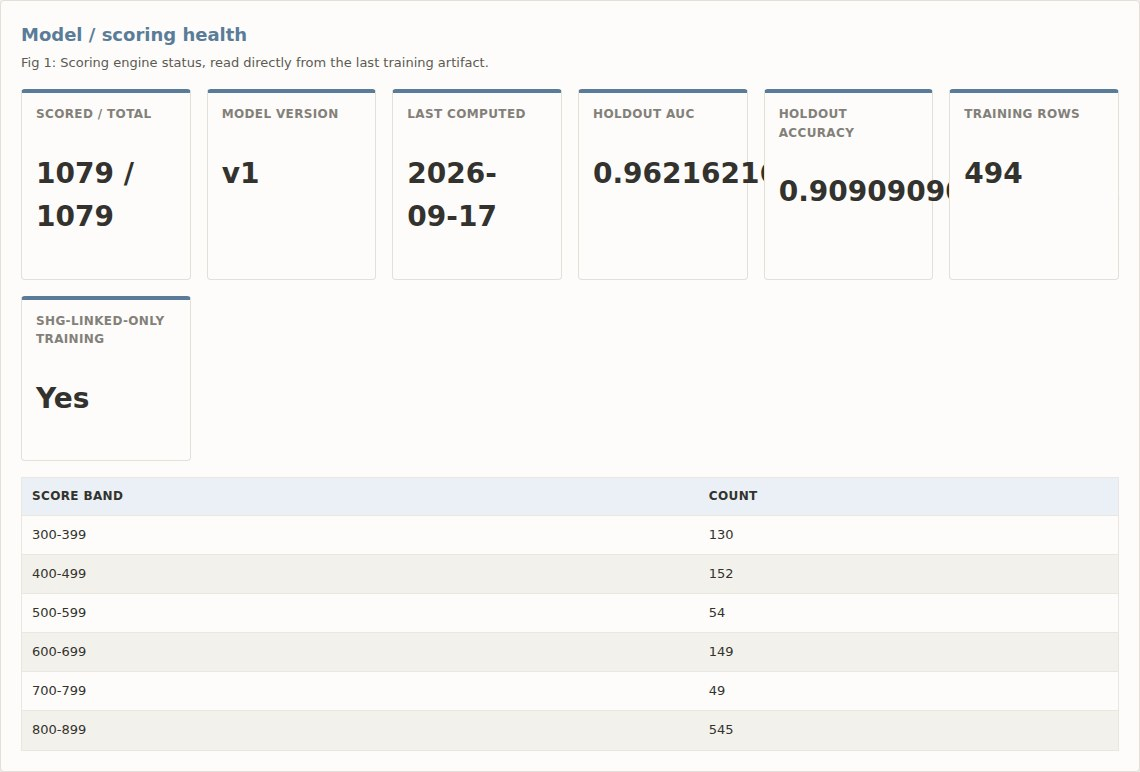
\includegraphics[width=\textwidth]{shots/ss_a_model.jpg}
\caption{Admin: model health}
\end{subfigure}
\caption{Lender, SHG and Admin screens}
\label{fig:ui2}
\end{figure}

\section{Analysis}
\label{sec:analysis}

\paragraph{Objectives met.} Seven of the eight objectives in
Table~\ref{tab:objectives} are fully met with measured evidence. The
eighth, automated validation, was met at the prototype stage, but the
suite is not stored with the code, so it could not be rerun after the
final changes.

\paragraph{Where the system exceeded expectations.} Every measured read
endpoint is at least an order of magnitude below the 300\,ms target except
the eligible-borrowers query (169\,ms), and the retrained model is both
better behaved and no less accurate than the one it replaced.

\paragraph{Challenges.} The most instructive problems were silent ones.
Nothing crashed when a fully repaid loan was offered for payment, when a
missed cycle could never be cleared, or when an on-time payment lowered a
score; each was found only by running a real flow and checking the
numbers against the database. The score problem in particular could not
be seen from any single score, only by comparing what the model did with
and without one extra payment.

\paragraph{How they were resolved.} Each data fix was paired with a
migration script that is safe to run twice and with a matching change to
the data generator, so a freshly seeded database does not bring the
problem back. The model change was tested on cross-validation before it
replaced the saved model, and the old model and database were backed up
first.

% ===== CHAPTER 4: CONCLUSION =====

\chapter{Conclusion}
\label{ch:concl}

\section{Summary of Work}

CreditSetu delivers a working, explainable, dual-path credit-scoring
engine; a formal SHG--lender partnership model; a two-directional loan
marketplace with targeted requests and lender reputation; four separately
authorised role-based views; and a live repayment flow whose effect on the
borrower's score has been verified end to end on the running system. The
final scoring model meets its accuracy targets (ROC-AUC 0.900, accuracy
0.853 on the holdout; 0.916 cross-validated ROC-AUC) and, unlike the model
it replaced, never lowers a score because of an on-time payment. All
measured read endpoints meet the response-time target.

\section{Key Findings}

\begin{itemize}
  \item \textbf{Monotonicity matters more than a few points of accuracy.}
  The unconstrained model had nearly the same ROC-AUC as the constrained
  one, yet it penalised on-time payments for almost one borrower in five.
  For a score that borrowers are told to improve, behaving consistently
  is a requirement in its own right.
  \item \textbf{A feature can be predictive and still wrong to use.}
  \code{n\_repayment\_events} carried real signal, but it measured how
  long a history is rather than how good it is, so every payment moved the
  score whatever its outcome.
  \item \textbf{Silent defects need end-to-end checks.} Every defect fixed
  in the final stage passed unnoticed through code review and through the
  prototype test suite; each was found by running the real flow and
  checking the stored numbers.
\end{itemize}

\section{Future Work and Recommendations}

\begin{enumerate}
  \item Commit the automated test suite to the repository, add cases for
  the per-loan wallet rule, the cycle rule and the monotone behaviour of
  the score, and run it on every change.
  \item Fix the two open defects (D-01, D-02) and replace the
  demonstration credential scheme with a vetted password library and
  short-lived signed tokens.
  \item Carry out the fairness sensitivity analysis of the gap between the
  independent (450) and SHG starting scores. It is a policy choice rather
  than something learned from data, and was planned for this report but
  not done.
  \item Decide how missed instalments should be handled. They are
  currently written off rather than carried as arrears, so 196 overdue
  loans that still have a balance cannot be paid through the app.
  \item Retrain on real data with a time-based train/test split, and
  retrain periodically as new repayments arrive.
  \item Integrate a real payment provider and EMI reminders, and build a
  mobile, multilingual interface for rural borrowers.
\end{enumerate}

\section{Final Remarks}

The project showed that a fair, explainable credit score for borrowers
without a formal history is achievable with mature open-source tools,
provided the score is held to the same standard a borrower would apply:
paying on time should never make it worse. The most valuable lessons came
from running the system end to end and comparing what it did with what it
should have done.

\section*{Data and Code Availability}
\addcontentsline{toc}{section}{Data and Code Availability}

The source code, documentation and synthetic data generator are available
at \url{https://github.com/shreesh1802/ucs503p-202627-Microfinance-Project}.

% ===== APPENDICES =====

\appendix

\chapter{Use Case Diagram}
\label{app:usecase}

Figure~\ref{fig:usecase} shows the four actors against every use case,
following UML~2.5~\cite{uml}. Viewing the score always includes generating
the improvement tips, and repaying an EMI always includes recomputing the
score, which is why a repayment cannot leave the score stale.

\begin{figure}[H]
\centering
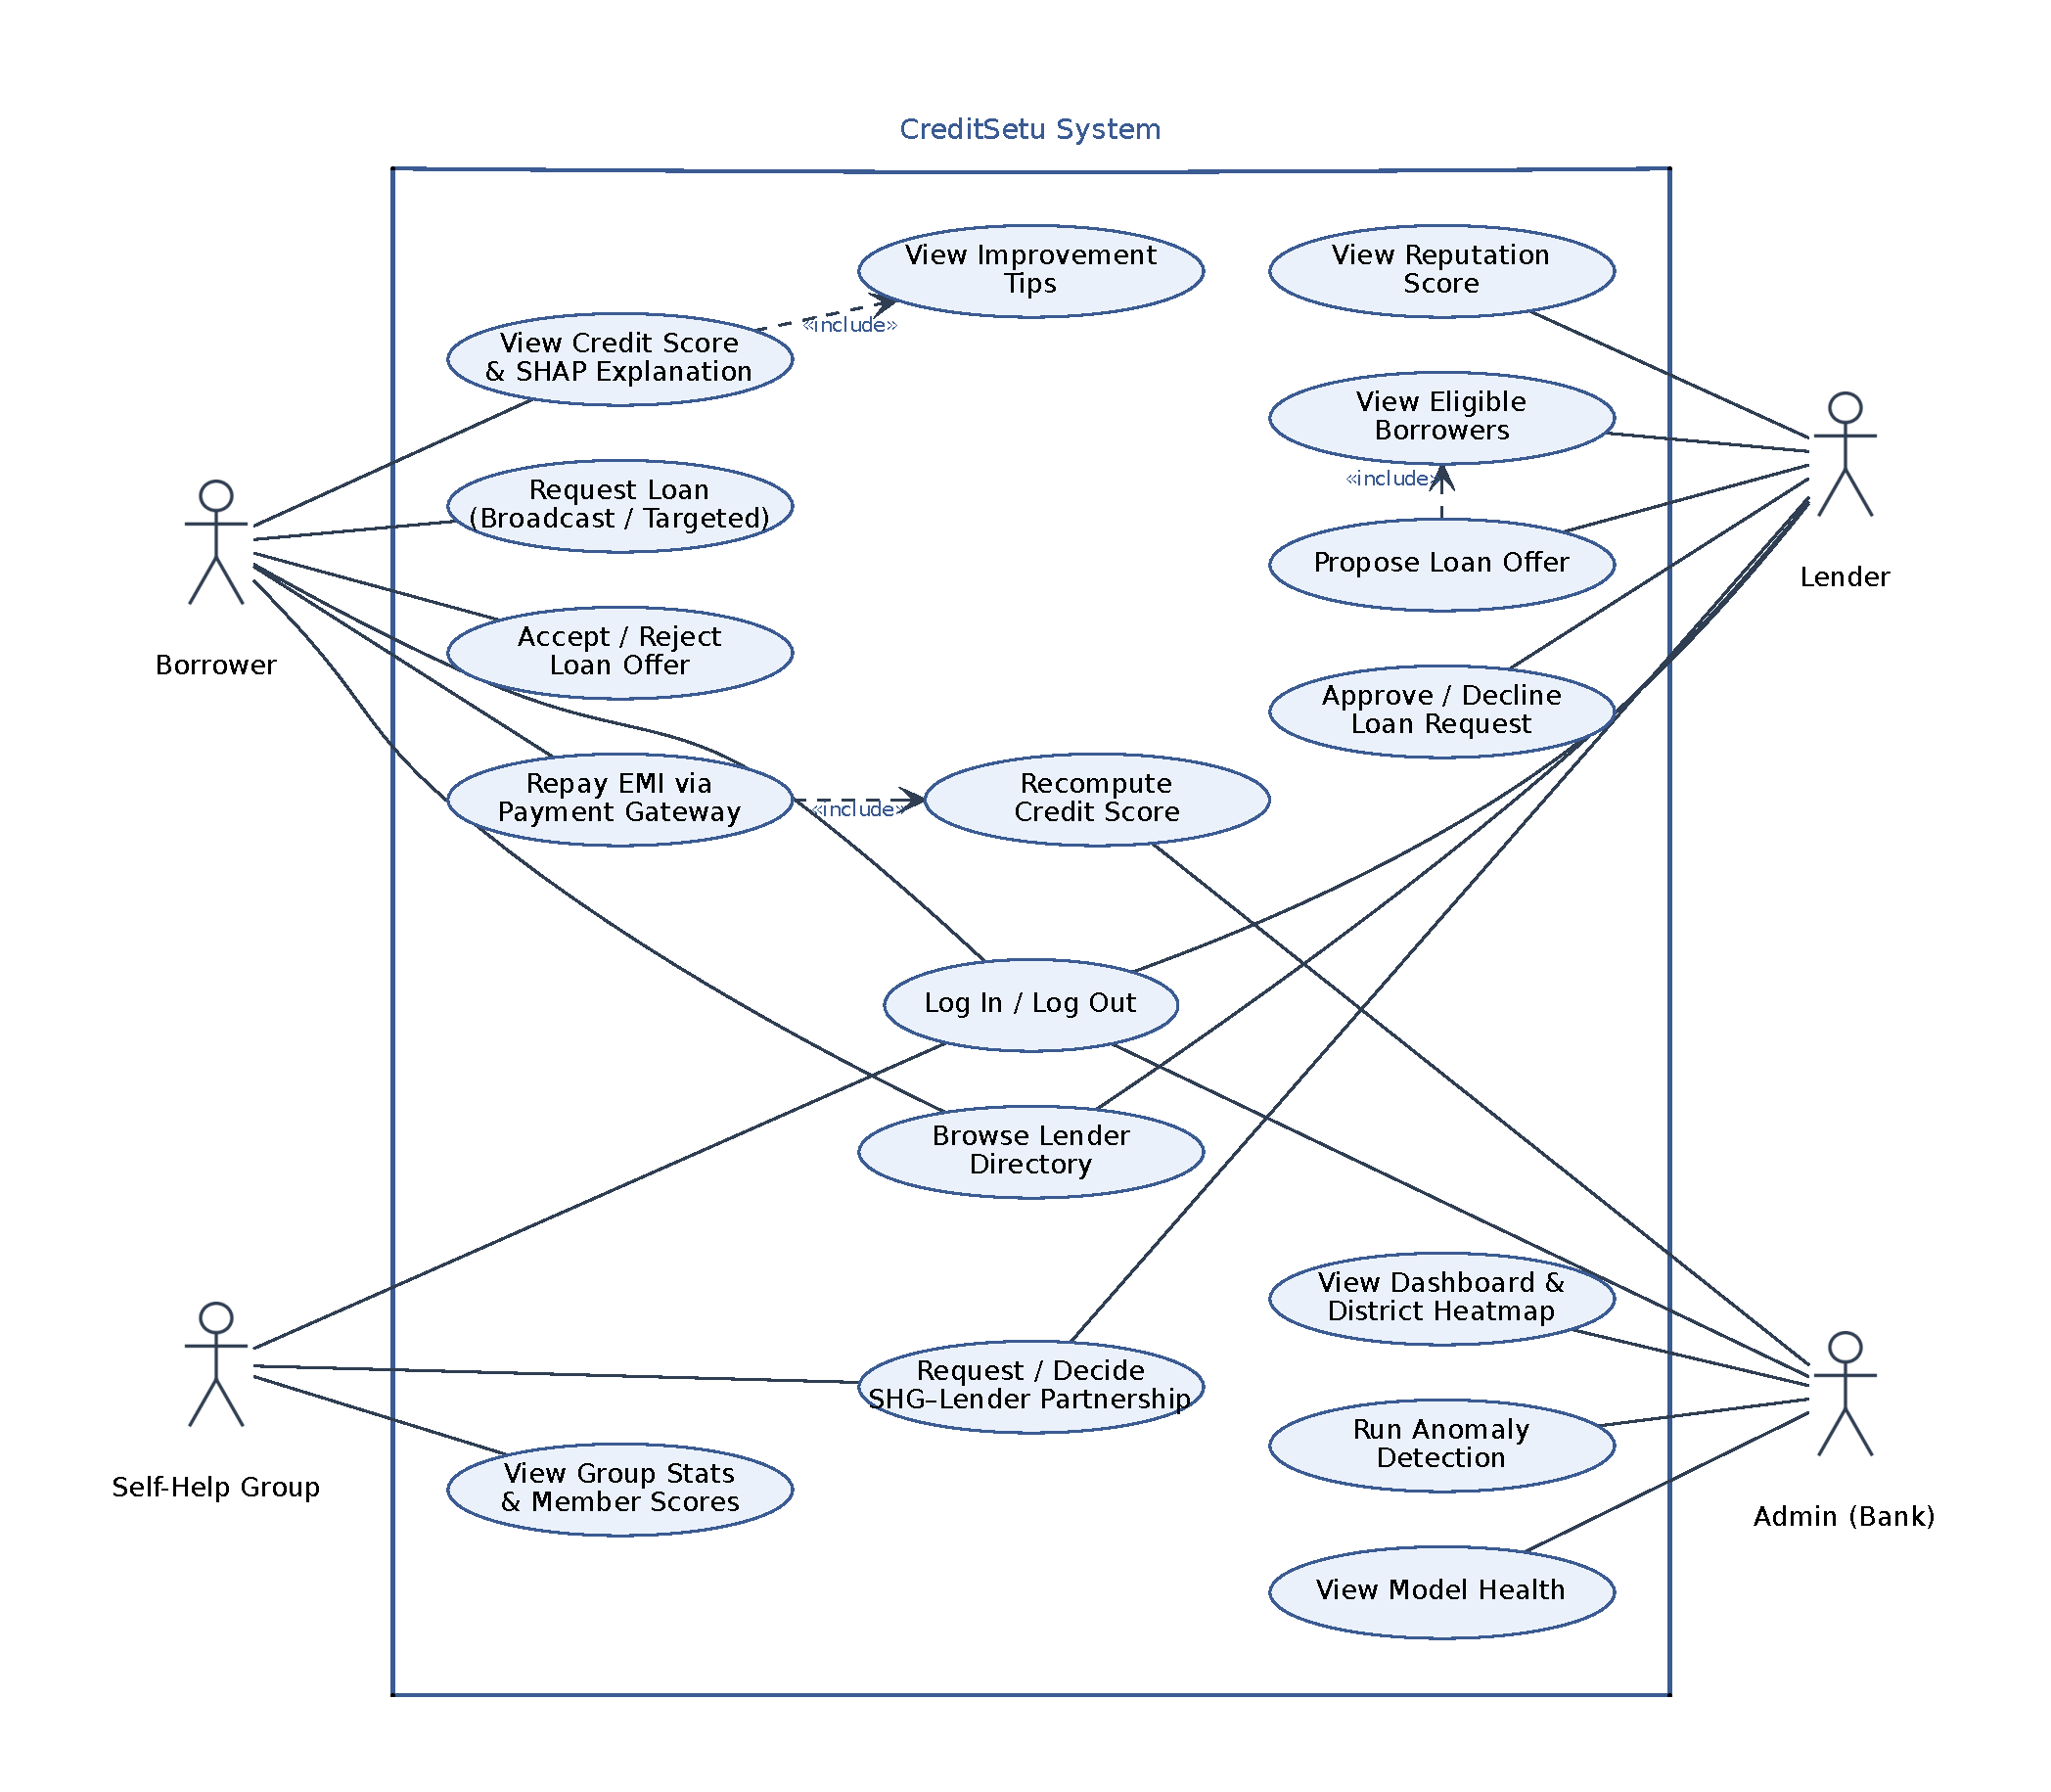
\includegraphics[width=\textwidth]{fig/use_case.pdf}
\caption{Use case diagram of CreditSetu}
\label{fig:usecase}
\end{figure}

\section*{Use Case Scenarios}
\addcontentsline{toc}{section}{Use Case Scenarios}

The HTTP status codes in the exception rows are the codes the API
actually returns.

\begin{table}[H]
\centering
\caption{Use case specification: Log In}
\small
\begin{tabular}{@{}L{2.8cm}L{10.4cm}@{}}
\toprule
\textbf{Use case} & UC01: Log In (role-gated)\\
\textbf{Actors} & Borrower, Self-Help Group, Lender, Admin\\
\textbf{Pre-conditions} & The account exists; the user has opened the login page for their role.\\
\textbf{Main flow} & (1) User submits credentials for one role. (2) System looks up the account for that role only. (3) System verifies the password against the stored salted PBKDF2 hash. (4) System creates a session row for that role and returns an opaque token valid for seven days. (5) The frontend opens that role's dashboard.\\
\textbf{Exceptions} & Unknown identifier or wrong password: 401, without saying which was wrong. A token used against another role's endpoints is refused.\\
\textbf{Post-conditions} & A session exists for exactly one role; the caller's identity for every later request comes from that session.\\
\bottomrule
\end{tabular}
\end{table}

\begin{table}[H]
\centering
\caption{Use case specification: View Credit Score and Explanation}
\small
\begin{tabular}{@{}L{2.8cm}L{10.4cm}@{}}
\toprule
\textbf{Use case} & UC02: View Credit Score, Explanation and Improvement Tips\\
\textbf{Actor} & Borrower (Admin may read any borrower's score)\\
\textbf{Pre-conditions} & Borrower is logged in and has at least one stored score.\\
\textbf{Main flow} & (1) System takes the borrower's id from the session. (2) System returns the latest score, its risk band and its basis (starting score, blended or model). (3) System returns the score history. (4) System returns the stored per-feature contributions in score points. (5) The dashboard shows them and turns the negative ones into up to five improvement tips.\\
\textbf{Exceptions} & Another borrower's score: 403. No token: 401.\\
\textbf{Post-conditions} & Nothing is modified.\\
\bottomrule
\end{tabular}
\end{table}

\begin{table}[H]
\centering
\caption{Use case specification: Request a Loan}
\small
\begin{tabular}{@{}L{2.8cm}L{10.4cm}@{}}
\toprule
\textbf{Use case} & UC03: Request a Loan (broadcast or targeted)\\
\textbf{Actor} & Borrower\\
\textbf{Pre-conditions} & Borrower is logged in and has a credit score.\\
\textbf{Main flow} & (1) Borrower enters principal, tenure and an optional purpose. (2) Borrower chooses broadcast or one eligible lender. (3) System checks the amounts and, for a targeted request, that the lender is still eligible. (4) System saves the request as Pending.\\
\textbf{Alternate flows} & Borrower retargets or withdraws a pending request.\\
\textbf{Exceptions} & Invalid amount or ineligible target: 400. Another borrower's request: 403.\\
\textbf{Post-conditions} & The request is in the queue of every eligible lender, or only of the target lender.\\
\bottomrule
\end{tabular}
\end{table}

\begin{table}[H]
\centering
\caption{Use case specification: Approve or Decline a Loan Request}
\small
\begin{tabular}{@{}L{2.8cm}L{10.4cm}@{}}
\toprule
\textbf{Use case} & UC04: Approve or Decline a Loan Request\\
\textbf{Actor} & Lender\\
\textbf{Pre-conditions} & At least one pending request is addressed to the lender, directly or by broadcast.\\
\textbf{Main flow} & (1) Lender opens its request queue. (2) Lender sees the borrower's score, risk band and path. (3) To approve, the lender enters an interest rate. (4) System re-checks eligibility and the lender's maximum loan amount at decision time. (5) System creates an Active loan.\\
\textbf{Alternate flows} & Declining hides the request from this lender only; it stays Pending for the others.\\
\textbf{Exceptions} & No interest rate: 400. Another lender's request, or an admin deciding: 403. Re-deciding: 400.\\
\textbf{Post-conditions} & Either an Active loan exists, or the request stays open for other lenders.\\
\bottomrule
\end{tabular}
\end{table}

\begin{table}[H]
\centering
\caption{Use case specification: Repay an EMI}
\small
\begin{tabular}{@{}L{2.8cm}L{10.4cm}@{}}
\toprule
\textbf{Use case} & UC05: Repay an EMI through the Demonstration Gateway\\
\textbf{Actor} & Borrower\\
\textbf{Pre-conditions} & Borrower is logged in, has an active loan with a cycle due and has signed in to the demonstration gateway.\\
\textbf{Main flow} & (1) System shows the wallet, the lender and EMI for each payable loan, and the total due. (2) Borrower clicks \emph{Pay this loan}. (3) System reloads the wallet and recomputes that loan's EMI and cycle on the server. (4) System records the payment as On\_Time or Late, debits the wallet, reduces the balance, and closes the loan after its last cycle or at a zero balance. (5) System recomputes the score and commits everything in one transaction. (6) The page shows the new score.\\
\textbf{Exceptions} & Wallet below this loan's EMI: 400 \code{insufficient\_funds} with both amounts. Loan not active: 400. Another borrower's loan: 403. Unknown loan: 404.\\
\textbf{Post-conditions} & Loan, wallet and score history change together, or not at all.\\
\bottomrule
\end{tabular}
\end{table}

\begin{table}[H]
\centering
\caption{Use case specification: SHG--Lender Partnership}
\small
\begin{tabular}{@{}L{2.8cm}L{10.4cm}@{}}
\toprule
\textbf{Use case} & UC06: Request or Decide an SHG--Lender Partnership\\
\textbf{Actors} & Self-Help Group, Lender\\
\textbf{Pre-conditions} & No approved or pending link already joins the two parties.\\
\textbf{Main flow} & (1) Either party sends a partnership request. (2) System stores it as Pending with the initiating role. (3) The other party approves or rejects it. (4) Once Approved, the lender may see the SHG's members and the members may target the lender.\\
\textbf{Alternate flows} & Either party may later revoke an approved partnership.\\
\textbf{Exceptions} & The initiating side deciding its own request, or an admin deciding: 403. A duplicate request or re-deciding: 400.\\
\textbf{Post-conditions} & Exactly one link row exists for the pair, with its state and initiating side.\\
\bottomrule
\end{tabular}
\end{table}

\chapter{Class Diagram}
\label{app:class}

Figure~\ref{fig:class} shows the domain model, which matches the
SQLAlchemy schema. \code{Individual.shg\_id} is optional, and a missing
value marks an independent borrower; this single nullable association
carries the whole dual-path design. \code{CreditScore} is append-only and
carries its own \code{ScoreExplanation} rows, so any past score and its
reason can be reconstructed. \code{SHGLenderLink} records its own state
and initiating side, which is what makes the approve/reject rule
enforceable. The \code{wallet\_balance} field added for the repayment flow
is not shown in this prototype-stage diagram.

\begin{figure}[H]
\centering
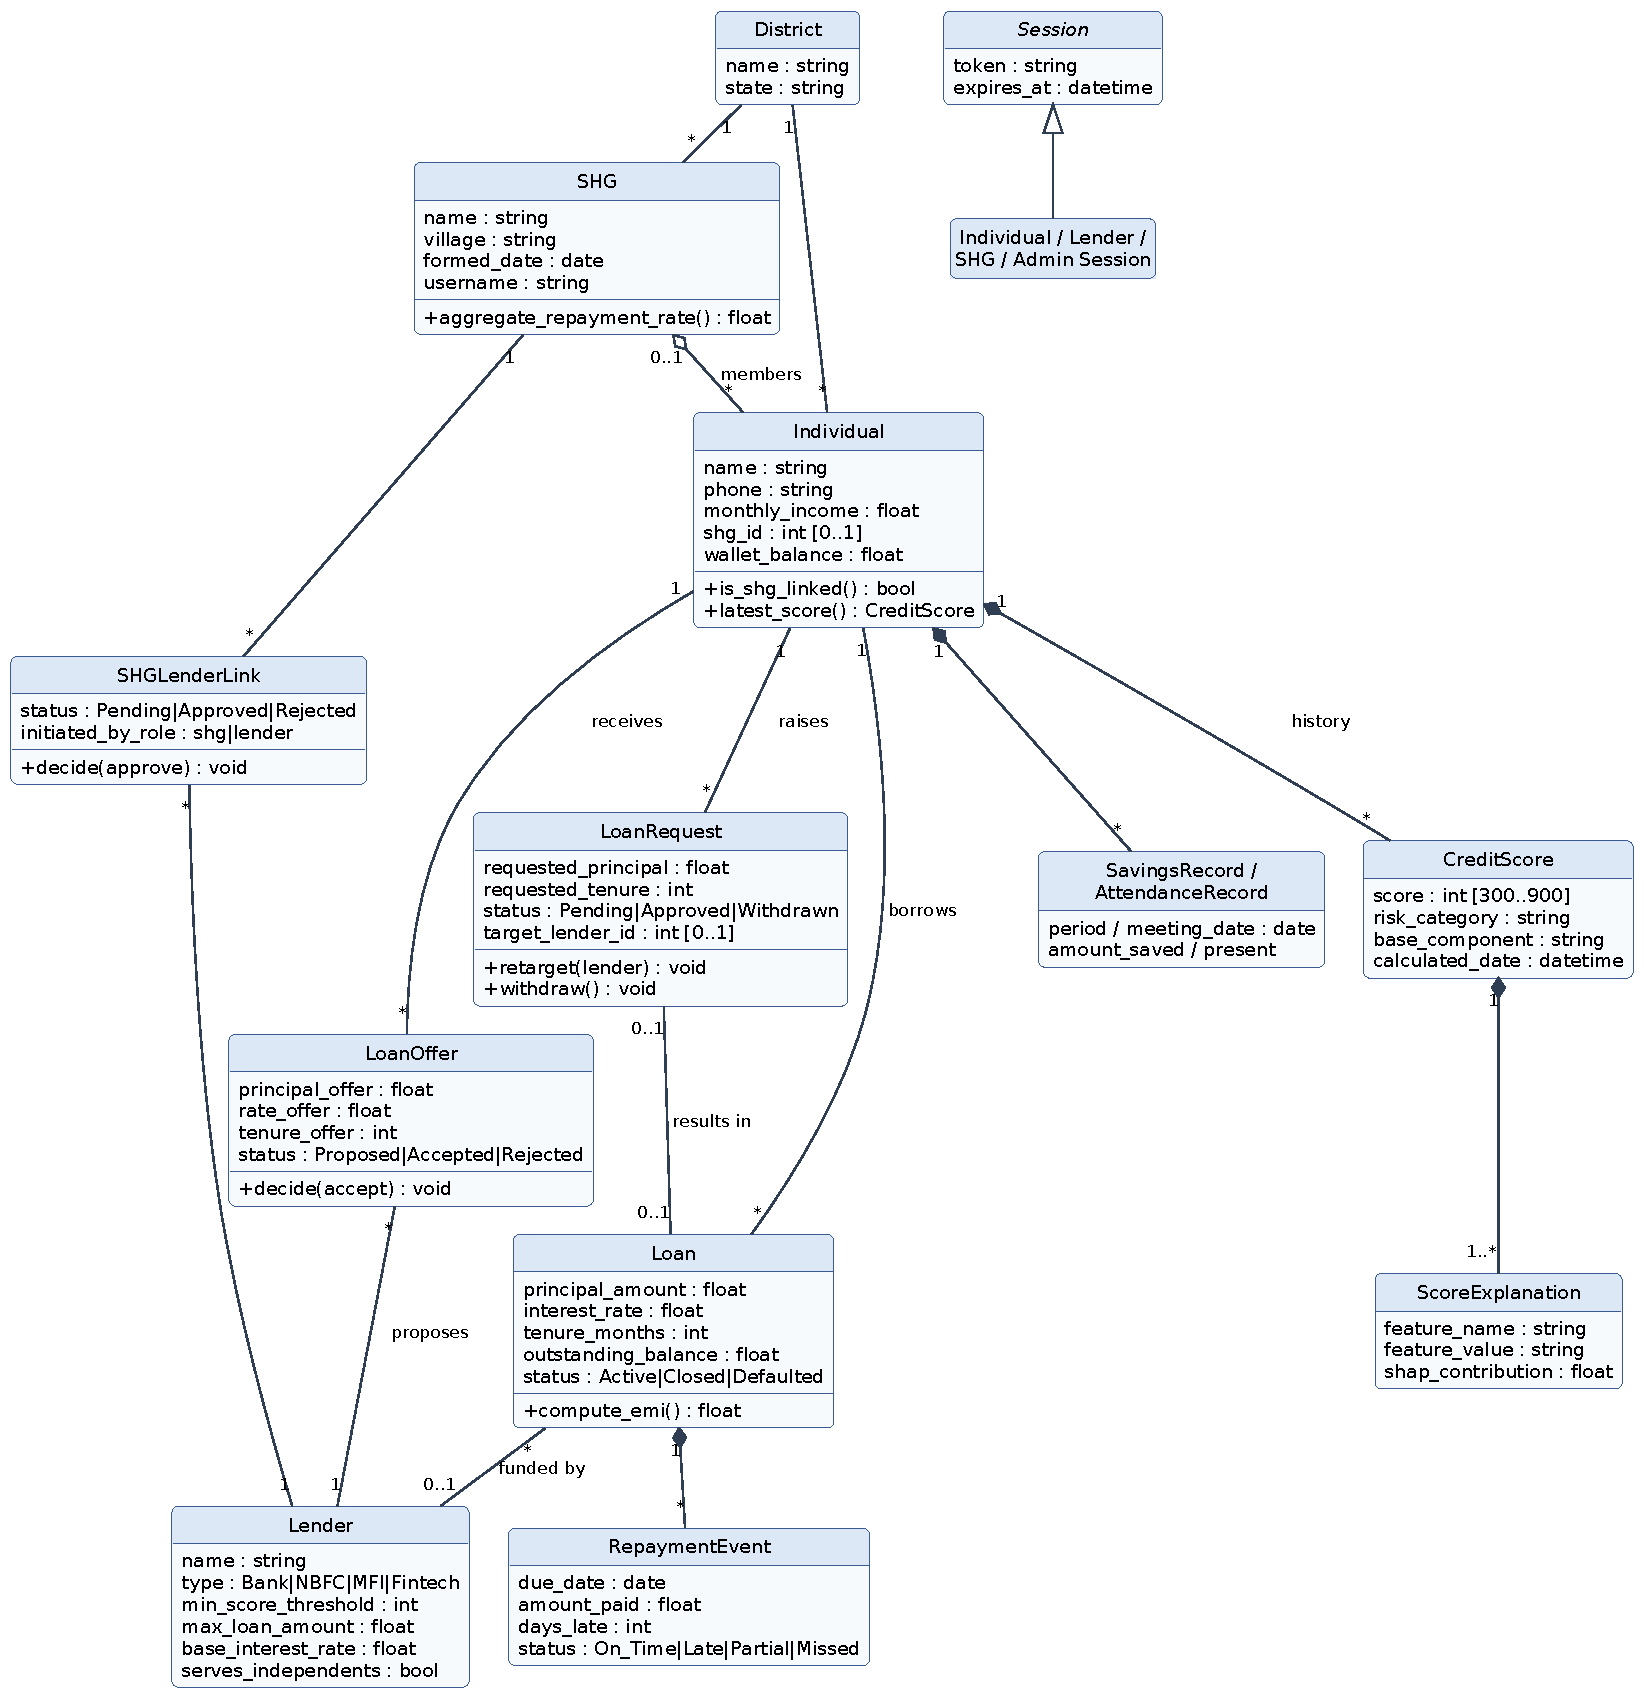
\includegraphics[width=\textwidth]{fig/class_c.pdf}
\caption{Class diagram (domain model)}
\label{fig:class}
\end{figure}

\chapter{Activity Diagrams}
\label{app:activity}

Figure~\ref{fig:activity} shows how a score is computed
(Section~\ref{sec:scoring}). The branch on SHG membership chooses the
starting score, and the branch on repayment history decides whether the
model is called at all. The diagram was drawn at the prototype stage and
still says 16 features; the final model uses 15
(Section~\ref{sec:monotone}). The flow is otherwise unchanged.

\begin{figure}[H]
\centering
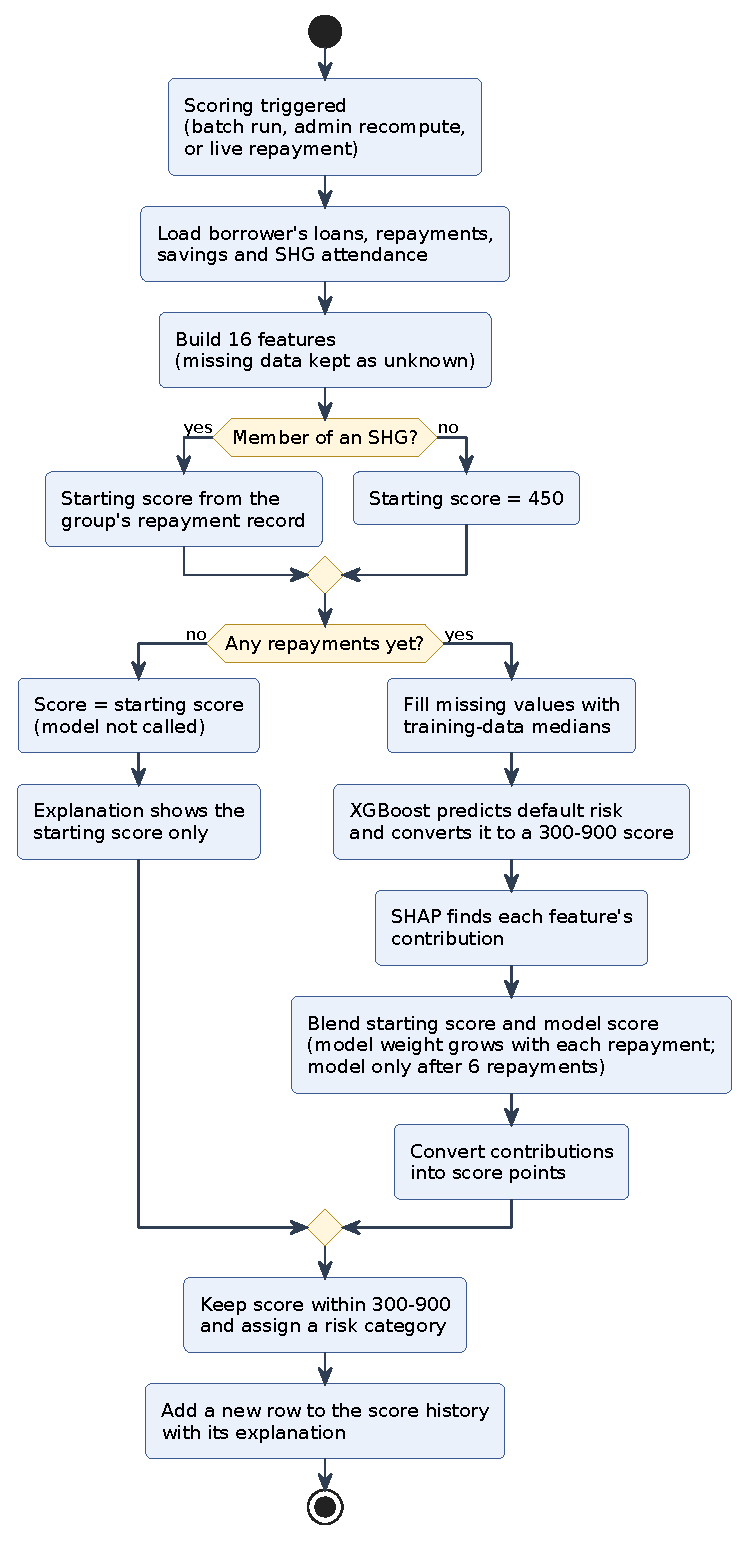
\includegraphics[height=0.72\textheight]{fig/activity_score.pdf}
\caption{Activity diagram: computing a borrower's credit score}
\label{fig:activity}
\end{figure}

Figure~\ref{fig:swimlane} shows the loan request, the lender's decision
and the repayment, one swimlane per participant. It was drawn at the
prototype stage: its wallet guard checks the total due across all loans,
whereas the final system checks each loan's EMI separately
(Section~\ref{sec:repay}).

\begin{figure}[H]
\centering
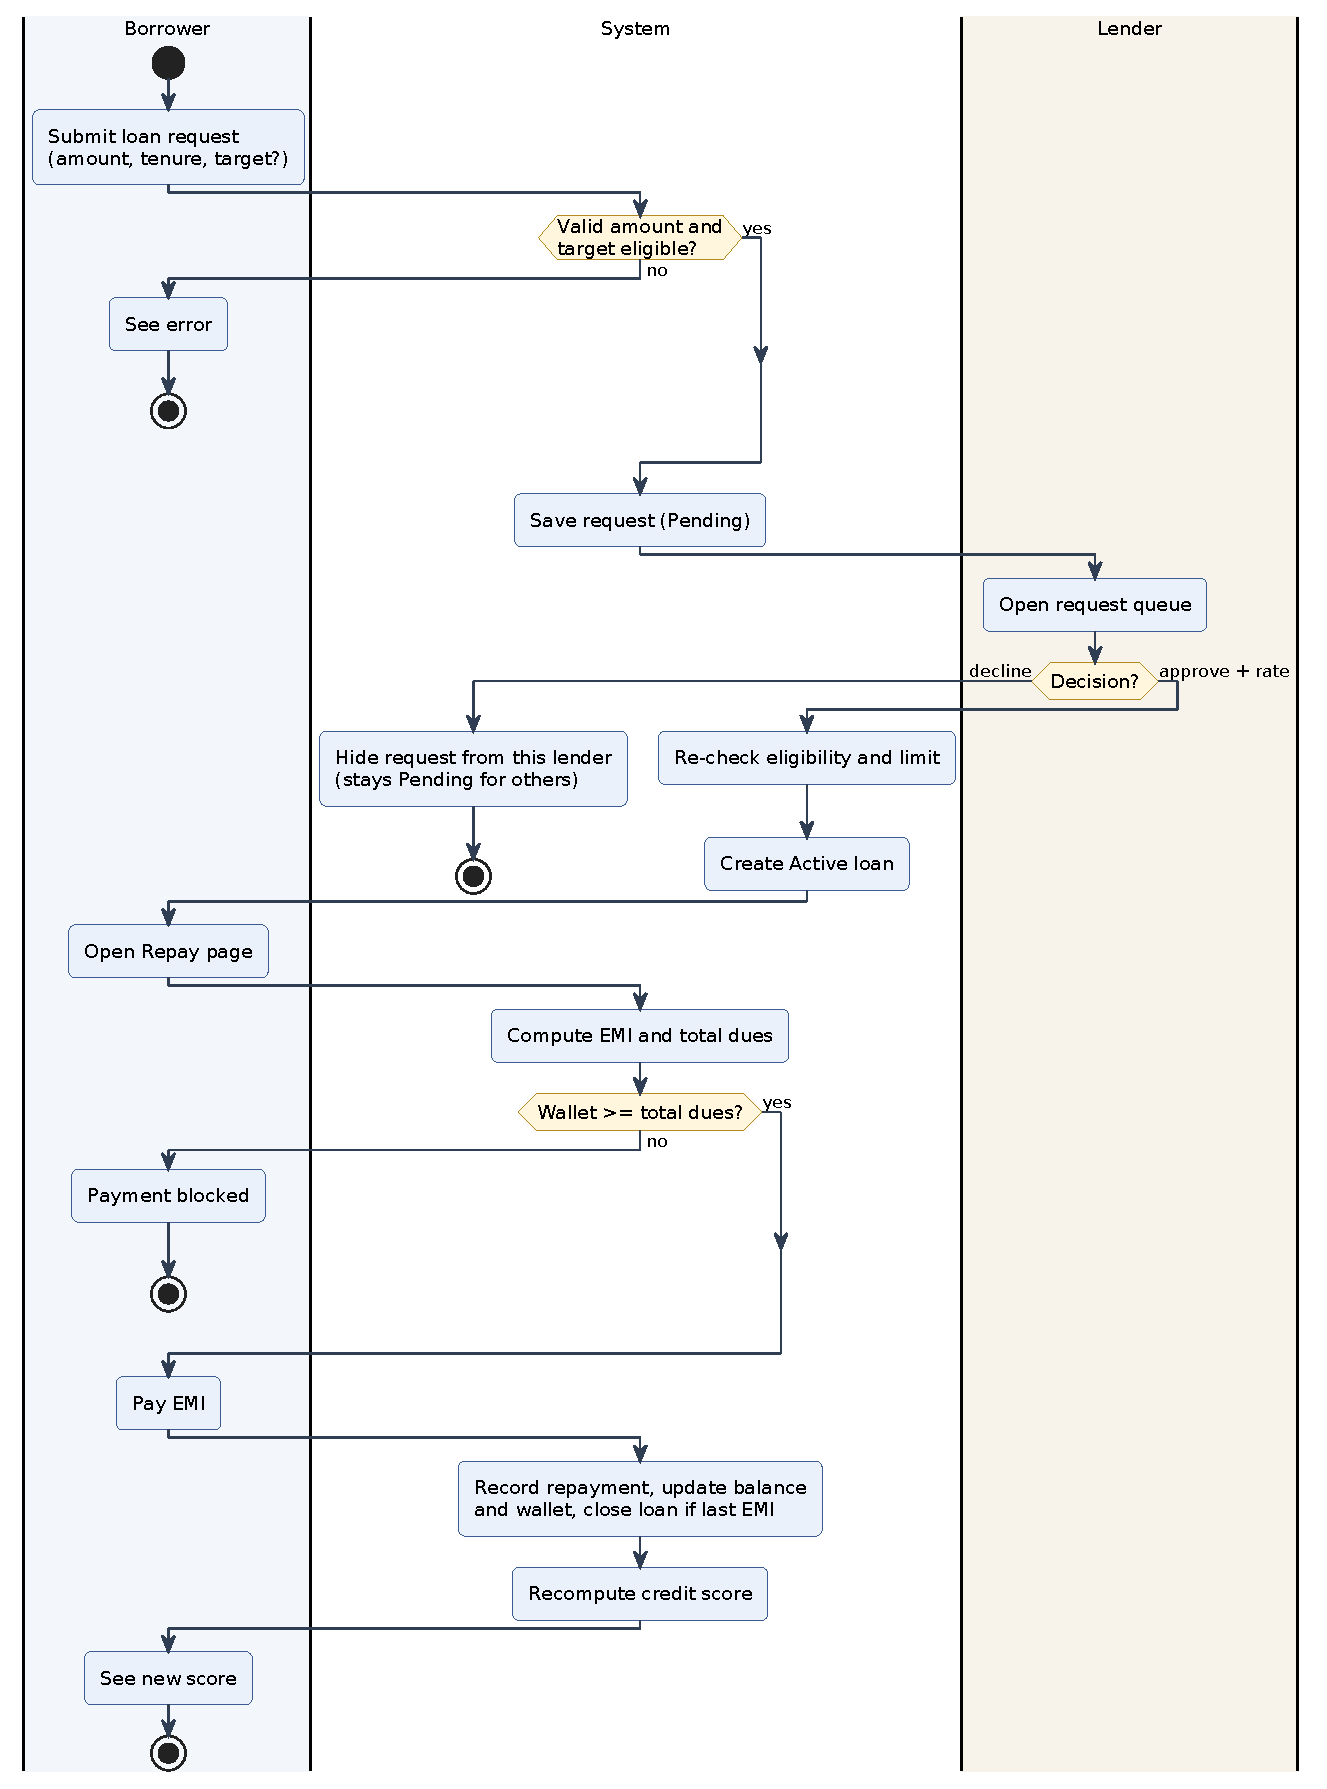
\includegraphics[height=0.72\textheight]{fig/swimlane_c.pdf}
\caption{Swimlane activity diagram: loan request, approval and repayment}
\label{fig:swimlane}
\end{figure}

% ===== BIBLIOGRAPHY =====

% Print bibliography with heading in TOC
\printbibliography[heading=bibintoc]

\end{document}
